\documentclass[oneside, letter, 12pt]{book}

% QCC book needs
\usepackage{fix-cm}  % this package allows large \fontsize
\usepackage{imakeidx}
\makeindex[title=Index]
\usepackage{listings}
\usepackage[table]{xcolor}

\usepackage{amsmath,graphicx}

\usepackage{tikz}    % this is for graphics. e.g. rectangle on title 
\usetikzlibrary{quantikz, decorations.pathmorphing,shapes.geometric}
%\usepackage{circuitikz}
\usepackage{tikz-3dplot} % includes tikz
\tdplotsetmaincoords{70}{120}


% This file is for commands / macros / functions.
% QCC book specific
\newcommand{\keta}[2][]{\vert {#2} \rangle_{#1}}
\newcommand{\braketa}[3][]{\langle {#2} \vert {#3}\rangle_{#1}}

\tikzstyle{Gate}=[rectangle, minimum width=30, minimum height=30, text width=20, text centered, draw=black]
% Content Starts Here
%%\chapter{About the Author}
Yuan John Jiang
\begin{document}
%% Cover page of the ebook. The ebook uses template developed by
%BSD 2-Clause License
%Copyright (c) 2021, Dominic Widdows
%All rights reserved.
%Redistribution and use in source and binary forms, with or without
%modification, are permitted provided that the following conditions are met:
%1. Redistributions of source code must retain the above copyright notice, this
%   list of conditions and the following disclaimer.
%
%2. Redistributions in binary form must reproduce the above copyright notice,
%   this list of conditions and the following disclaimer in the documentation
%   and/or other materials provided with the distribution.

\thispagestyle{empty}

\vspace{3cm}
  \begin{center}
	\bfseries \Huge \latex Quantum Information, Algorithms and Protocols \par   % Your own title would go here.
        ~\\
	\bfseries \LARGE A Textbook for Computer Science and Engineering Students \\   % Include a subtitle or just delete.
        ~\\
        \bfseries \Large Yuan John Jiang \par   % The author's name goes here.

        \vspace{3cm}
    
%      	{\centering \includegraphics[width=0.8\linewidth]{images/cover.png}}
    \end{center}
    
\par

\newpage



% The asterisk excludes chapter from the table of contents.
\addcontentsline{toc}{chapter}{Preface}
\chapter*{Preface}
Quantum computing and communication are hot topics. Software development kits (SDKs) including IBM Qiskit and Google Cirq have been made available to software engineers. But they are useless if the engineers are not trained with quantum algorithms and protocols, which have been described as mysterious and incomprehensible. Can engineers be taught the algorithms and protocols without studying quantum physics? After all, the Nobel prize-winning physicist and one of the best educators, Richard Feynman, says “I think I can safely say that nobody really understands quantum mechanics.”

This book says "Yes!" The only concept that one needs to learn about quantum physics is that at the minuscule scale, a wave cannot be divided into any smaller portions in terms of its energy or mass. The rest of the undergraduate courses on quantum physics are about solving Schrödinger equation for electron waves. But we all use Wi-Fi, cellular, cable, and optical fiber communications daily, which use electromagnetic waves underneath. Communication engineers can even design communication systems including protocols without learning how to solve wave equations. They do need to learn modulation theory though, which studies how information can be carried or represented by wave parameters. It is the key to linking waves to information. Communication and software engineers just need to study or review modulation theory in the context of quantum waves to understand quantum algorithms and protocols, and hopefully to be able to invent new ones.

\section{Arrangement of this book}
The first chapter \ref{c-intro} gives an overview of quantum technologies. The next chapter \ref{c-modulation} on classical modulation theory serves as a foundation for the quantum information discussion of chapter \ref{c-qinfo}. Quantum information differs from the classical theory because of the limitation of quantum measurement. Chapter \ref{c-comm} studies several quantum communication protocols, which use one to three qubits and are easy to understand. The rest focus on several n-qubit algorithms including Shor's algorithm and are arranged by design patterns. If any reader is interested in knowing how quantum qubits and gates work at the physical level, Appendix \ref{A-qubit} is reserved for this subject.

% Three-level Table of Contents
\setcounter{tocdepth}{3}
\tableofcontents

\mainmatter

\chapter{Introduction}\label{c-intro}
The advantage of quantum computing lies in the possibility of parallel computing.

\section{The power of parallel computing}
Maze\index{Maze} problems are hard because there are too many paths to explore from the entrance to the exit. If changing the question of the problems from pinpointing the actual paths to finding the number of good paths, although seemingly dumb down, the challenge is as hard as the original. One still needs to explore all the possible paths to reach the conclusion.

\begin{figure}[h]\label{Maze}
%\includegraphics[width=6cm]{pic/maze.png}
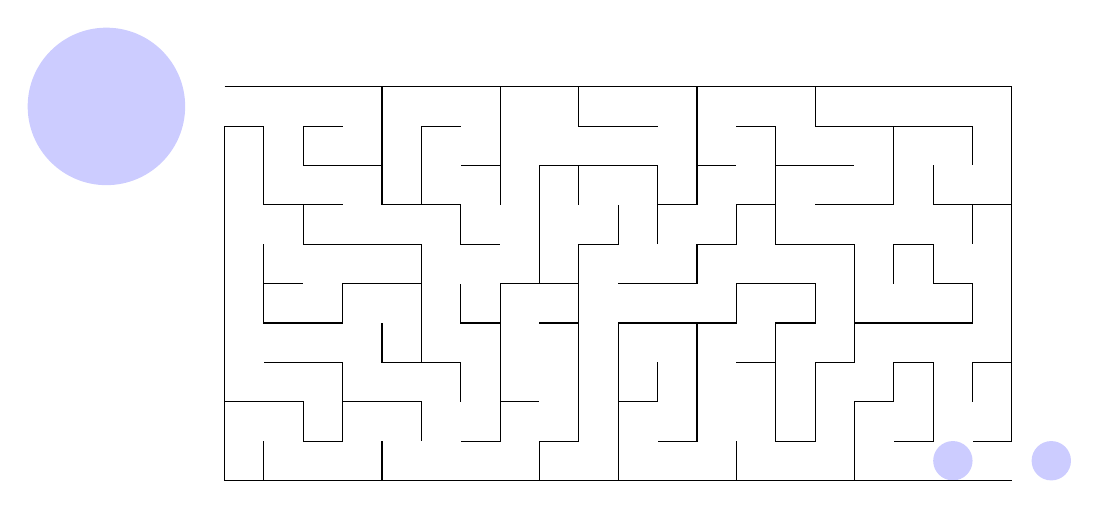
\begin{tikzpicture}[scale=0.5]
% Water
\fill[blue!20] (-3,9.5) circle (2);
\fill[blue!20] (18.5,0.5) circle (0.5);
\fill[blue!20] (21,0.5) circle (0.5);
%\fill[red!30] (13.5,2.2) circle (0.5);
%\fill[blue!20] (15.5,3.8) circle (0.5);

% outer lines
\draw (0,10) -| (20,1) -- +(-1,0);
\draw (20,0) -| (0,9) -| (1,7) -- (3,7);
\draw (2,7) |- (5,6) |- (6,3) -- (6,2);
\draw (5,3) -| (4,4);
\draw (5,5) -| (3,4) -| (1,6); \draw (1,5) -- (2,5);

% bottom row
\draw (0,2) -| (2,1) -| (3,3) -- (1,3); \draw (3,2) -| (5,1);
\draw (1,0) -- (1,1);
\draw (4,0) -- (4,1);
\draw (8,0) |- (9,1) |- (10,6) -- (10,7); \draw (8,4) -- (9,4); \draw (8,5) -- (9,5);

\draw (10,0) |- (13,4) |- (15,5) |- (14,4) |- (15,1) |- (16,3) |- (14,6) |- (13,9);
\draw (10, 2) -| (11,3); \draw (12,4) |- (11,1); \draw (13,3) -- (14,3);
\draw (16,4) -| (19,5) -| (18,6) -| (17,5);
\draw (14,7) -| (13,6) -| (12,5) -- (10,5); \draw (14,8) -- (16,8);

\draw (13,0) -- (13,1);
\draw (16,0) |- (17,2) |- (18,3) |- (17,1);
\draw (20,3) -| (19,2);

% top row
\draw (4,10) |- (6,7) |- (7,6); \draw (4,8) -- (2,8) |- (3,9); \draw (5,7) |- (6,9);
\draw (7,10) -- (7,7); \draw (7,8) -- (6,8);
\draw (9,10) |- (11,9);
\draw (12,10) |- (11,7); \draw (11,6) |- (8,8) |- (7,5) |- (6,1);
\draw (12,8) -- (13,8); \draw (9,8) -- (9,7); \draw (7,4) -| (6,5); \draw (7,2) -- (8,2);
\draw (15,10) |- (19,9) -- (19,8); \draw (17,9) |- (15,7);
\draw (20,7) -| (18,8); \draw (19,7) -- (19,6);
\end{tikzpicture}
\caption{Maze}
\end{figure}

Computer scientists have long known parallel computing\index{parallel computing} is the way to speed up solutions to such problems. But how to realize parallel computing needs the help of physicists. Indeed, a physicist would suggest the following experiment to attack the problem: run water into the entrance and observe what's coming out of the exit. If we see water out of the exit, we know the maze has at least one good path.

We can obtain more information if we explore the water experiment further: put several drops of water into the entrance at the same time and observe which drop comes out first or last. Apparently, the time lapse between a drop's entrance to exit carries the length information of the path, which it travels. But what happens if two drops come out at the same time? Clearly, the traveling time of a water drop alone is not sufficient to extract more information from the maze.

The clever physicist may suggest adding color to the experiment: design a mechanism so that a water drop is stained with a different color when it is bounced back from a dead-end. When we see a purple drop twice as big exiting, we can be sure that it is a mixture of two drops, one being bounced back from a dead-end and stained red, and the other has remained blue.

The above thought experiment demonstrates that a medium can be used for parallel exploration or information processing if
- it can spread and propagate multiple paths in parallel and
- it can be broken up into the smallest drops with each carrying its own piece of information.
Water is a familiar medium we use every day but is far from ideal for the parallel computing jobs we hope to do. Physicists have better media to use: quantum waves. One big problem with water is that a water drop can always be divided into smaller ones, and we are never sure whether it is a combination of several smaller drops. Not only that, it loses liquidity quality when a drop gets down to the level of hundreds of molecules. In contrast, a drop of quantum wave is the smallest and cannot be divided. And the spreading or propagating quality is independent to the number of drops. If we can separate quantum waves into controllable drops with each carrying a piece of information, we may process the information carried by the drops in parallel.

\begin{figure}[h]\label{MazeStain}
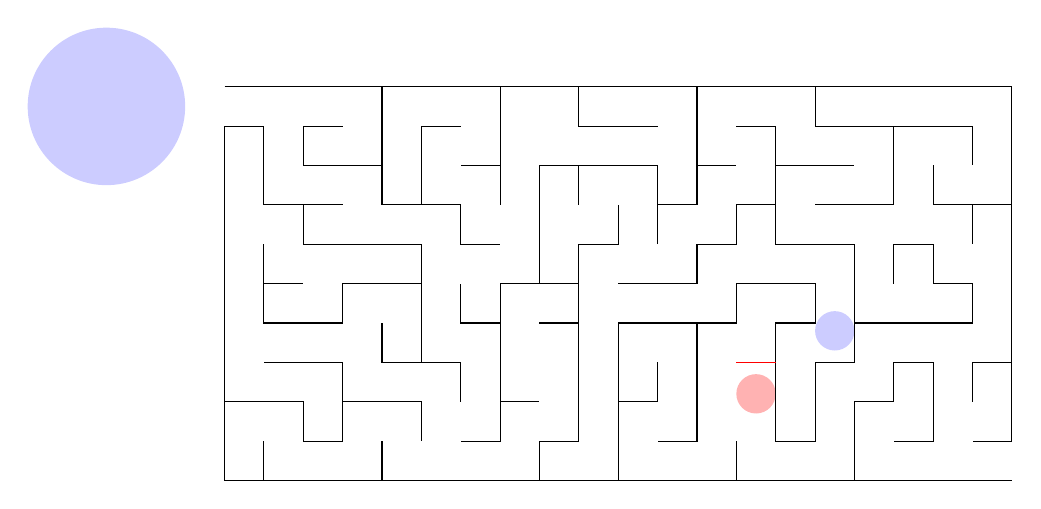
\begin{tikzpicture}[scale=0.5]
% Water
\fill[blue!20] (-3,9.5) circle (2);
%\fill[blue!20] (18.5,0.5) circle (0.5);
%\fill[blue!20] (21,0.5) circle (0.5);
\fill[red!30] (13.5,2.2) circle (0.5);
\fill[blue!20] (15.5,3.8) circle (0.5);

% outer lines
\draw (0,10) -| (20,1) -- +(-1,0);
\draw (20,0) -| (0,9) -| (1,7) -- (3,7);
\draw (2,7) |- (5,6) |- (6,3) -- (6,2);
\draw (5,3) -| (4,4);
\draw (5,5) -| (3,4) -| (1,6); \draw (1,5) -- (2,5);

% bottom row
\draw (0,2) -| (2,1) -| (3,3) -- (1,3); \draw (3,2) -| (5,1);
\draw (1,0) -- (1,1);
\draw (4,0) -- (4,1);
\draw (8,0) |- (9,1) |- (10,6) -- (10,7); \draw (8,4) -- (9,4); \draw (8,5) -- (9,5);

\draw (10,0) |- (13,4) |- (15,5) |- (14,4) |- (15,1) |- (16,3) |- (14,6) |- (13,9);
\draw (10, 2) -| (11,3); \draw (12,4) |- (11,1);
 \draw[red] (13,3) -- (14,3);
\draw (16,4) -| (19,5) -| (18,6) -| (17,5);
\draw (14,7) -| (13,6) -| (12,5) -- (10,5); \draw (14,8) -- (16,8);

\draw (13,0) -- (13,1);
\draw (16,0) |- (17,2) |- (18,3) |- (17,1);
\draw (20,3) -| (19,2);

% top row
\draw (4,10) |- (6,7) |- (7,6); \draw (4,8) -- (2,8) |- (3,9); \draw (5,7) |- (6,9);
\draw (7,10) -- (7,7); \draw (7,8) -- (6,8);
\draw (9,10) |- (11,9);
\draw (12,10) |- (11,7); \draw (11,6) |- (8,8) |- (7,5) |- (6,1);
\draw (12,8) -- (13,8); \draw (9,8) -- (9,7); \draw (7,4) -| (6,5); \draw (7,2) -- (8,2);
\draw (15,10) |- (19,9) -- (19,8); \draw (17,9) |- (15,7);
\draw (20,7) -| (18,8); \draw (19,7) -- (19,6);
\end{tikzpicture}
\caption{Maze with stained water drops}
\end{figure}

\section{The quantum power}
As a matter of fact, all waves at low levels of energy or mass are quantum waves. Quantum physics claims all waves have their smallest drops -- the quanta\index{quanta}, which cannot get any smaller when measured by their energy or mass. Einstein was the first to hypothesize this nature of light, which scientists had assumed since Christiaan Huygens' time: its energy could be dimmed as low as one wishes. The very word "quantum"\index{quantum} suggests this concept. This is often called the particle nature of waves. But as we will explain below, calling it the quantum nature is more precise.

Einstein's discovery, a hypothesis at the time, might have something to do with his prior discovery, which equates mass with energy. Until then, all matter had mass and is composed of elementary particles. Einstein's revelation that light is also matter, which has only energy, is a precursor of the revelation that all matter is fundamentally wave. Bohr was the first to hypothesize the wave nature of electrons, which had only been known as particles.

The complete theory of quantum physics can be summarized by the particle and wave dual nature of matter:
- all matter is waves and
- each wave's energy or mass is an integer number of its smallest unit.
These two concepts are the essence of quantum physics. Quantum theory has been successfully applied to the invention and advancement of many modern technologies, including lasers and semiconductors. But the devices typically comprise of matter million to quadrillion quanta in term of energy or mass. Even the tiniest transistor device in a modern semiconductor chip comprises at least thousands of electrons. Nevertheless, advances in modern technologies have getting us close to work with waves at the individual quantum level.

The idea of using the parallel computing power of quantum waves is not new. The publication of Deutch's algorithm\index{Deutsch's algorithm}\cite{1985Deutsch} in 1985 did not garner much attention. But the publication of Shor's algorithm\index{Shor's algorithm} in 1997, which may be considered an extention of Deutsch's, shocked the world with its potential power of factoring large numbers and consequently breaking modern encryption technologies.

The idea of applying quantum technology to secure communication came in 1984 with the publication of BB84 protocol\cite{BB84}. The idea is simple: using waves with one quantum of energy in each to transmit information. Since a wave of one quantum cannot be divided and therefore, it cannot be partially tapped for eavesdropping.

\subsection{The wave nature}
\begin{figure}[h]\label{String}
%\includegraphics[width=6cm]{pic/wave-in-a-string.png}
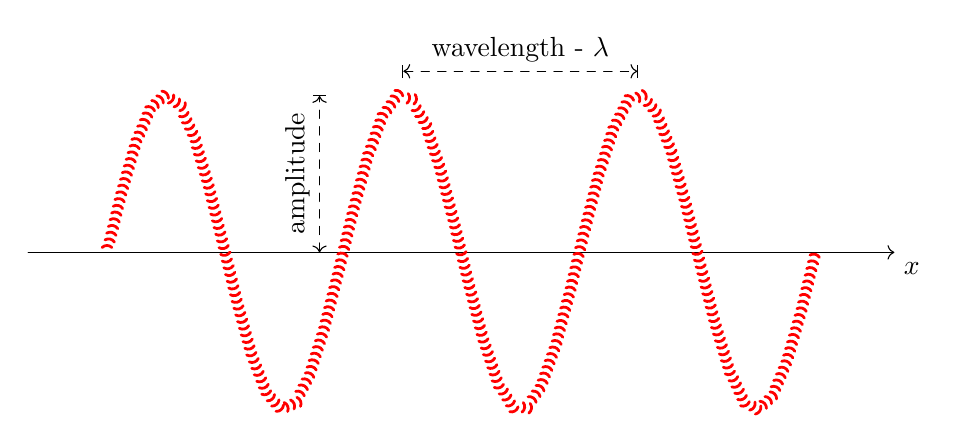
\begin{tikzpicture}[line join=round, line cap=round]

  % draw coordinate
  \draw[->] (-1,0) -- (10,0) node[pos=1.02,below] {$x$};
 % \draw[->] (0, -1) -- (0,2);
  % Rope properties
  \def\length{9}  % Length of the rope
  \def\thickness{1}  % Thickness of the rope
  \def\waveAmplitude{2}  % Amplitude of the wave
  \def\waveLength{3}  % Wavelength
  \def\segments{50}  % Number of segments
  
  % Draw the rope
  \draw[decorate, decoration={waves, segment length=2.5}, line width=\thickness, red]
    (0,0) -- plot[domain=0:\length, samples=\segments]
    (\x, {\waveAmplitude*sin(\x*(360/\waveLength))}) -- (\length,0);

    % label
    %\draw[red, fill] (3.75,2) circle(0.05cm);
    %\draw[red, fill] (6.75,2) circle(0.05cm);
    %\draw[dashed] (2,2) -- (3.75,2);
    \draw[<->|, dashed] (2.7,0) -- (2.7,2) node[pos=0.5, rotate = 90, above] {amplitude};
    \draw[|<->|, dashed] (3.75,2.3) -- (6.75,2.3) node[pos=0.5, above] {wavelength - $\lambda$};

\end{tikzpicture}
\caption{Wave arose from shaking or vibrating a string.}
\end{figure}

When talking about waves, we often visualize ripples in a lake or the surges in oceans and seas. We observe water being pushed up and then pulled down by gravity. If we shake one end of a string, as shown in Fig. \ref{String}, we can observe that each section of the string vibrates, and the vibration propagates from close to far. Vibration\index{vibration} in time and propagation\index{propagation} in space are the fundamental features of all waves. But can we consider the vibration of a guitar string as a wave? Indeed, we can. The reason why we do not perceive propagation is that the propagation gets reflected back and forth by the two fixed ends of the string. Therefore, propagation remains a defining feature of waves, even if their propagation is constrained in the spatial dimensions.

Quantum computing and communication use only electromagnetic waves and electron waves. Electromagnetic waves are the vibration of electric and magnetic fields. We are already familiar with radio waves and light waves used in Wi-Fi, cellular, cable, and optical fiber communications, as they are part of our daily lives. However, we do not see the quantum nature of these waves because each has quadrillions or more quanta flowing per second. We only see the average effect.

The vibration of an electron wave is not visible like that of a vibrating string or directly measurable like an electromagnetic wave. However, physicists do find sufficient evidence of the vibration and discovered Schrödinger equation to describe it. In addition, Thomson's double slit experiment\cite{THOMSON} shows that the vibration propagates. Moreover, modern-day semiconductor and superconductor technologies could not be realized without the wave nature of electrons.

\subsection{The particle nature}
To most people, particles have the image of point-like things with negligible sizes but observable locations. This image is wrong and is the cause of many misunderstandings about quantum physics. A water drop has no precise size or location because it spreads everywhere in a container. Similarly, a quantum wave spreads or propagates to everywhere unless something contains it. Except for energy and mass, the particle nature of matter does not relate to any of the characteristics that people typically associate with particles. It really should be referred to as the quantum nature.

Among all quantum waves, only electromagnetic waves and electrons are relevant to quantum technologies. For electromagnetic waves, including lights, measuring their energy shows the smallest quanta and each quantum is called a photon. The challenge to hardware scientists and engineers is to be able to separate and isolate individual photons or electrons so that each can carry information and, at the same time, to keep them synchronized so that they can be transformed as one wave to achieve parallel processing. Appendix \ref{A-qubit} explains the physics behind some of the techniques. Otherwise, this book will not go into any deeper in physics.

\section{Constructing a quantum computer}
Quantum computing uses quantum waves to process information. But in the real world, there is no such thing as a quantum computer that is built entirely with quantum waves. Only certain portions of the circuits of an otherwise conventional computer operate with quantum waves. One interacts with the computer just like with any other computer. One even programs on a conventional computer and uses languages such as Python. Only the portion of a program that requires parallel computing invokes a quantum circuit. For example, the following code starts by importing the class "QuantumCircuit" from package "qiskit" provided by IBM.
\begin{lstlisting}
from qiskit import QuantumCircuit

c = QuantumCircuit(2, 2)
c.h(0)
c.cx(0, 1)
c.measure(0, 0)
c.measure(1, 1)    
\end{lstlisting}
The code is the beginning portion of a program implementing the superdense protocol for encrypted communication illustrated in Fig. \ref{denseCoding}. It is a good example to show the essential components of a quantum system.

Despite being in Python, a high-level language, the following lines of the code relating to quantum computing are more like programming at the assembly language level, at which programmers worked 50 years ago:
\begin{itemize}
\item line 3 creates a quantum circuit object with 2 quantum registers and 2 conventional computer registers to store information; the registers are always initialized to be "0" upon creation;
\item line 4 connects the first quantum register labeled as "0" to an "H" quantum gate, which reads the information from the register, changes it, and puts the result back into the register;
\item line 5 connects the two quantum registers labeled as "0" and "1" to a "CX" quantum gate, which reads their information, changes it, and puts the result back into the registers;
\item line 6 connects the first quantum register to a "Measure" gate, which reads from the quantum register and outputs to the conventional register labeled as "0";
\item line 8 repeats the previous step for the second quantum and conventional registers.
\end{itemize}

In the standard von Neumann computer architecture, a register\index{register} is an information memory device; and a gate is an information processing device. A processing unit\index{processing unit} is a circuit connecting the two types of devices. A quantum processing unit also adheres to this von Neumann architecture. Fig. \ref{Circuit} is a quantum circuit diagram\index{quantum circuit diagram} implementing the above program. Each line in the diagram is a quantum register called a quantum bit (qubit)\index{qubit} whose wave parameters are initialized to represent zero. "H" and "CX" gates are drawn as rectangular boxes in the diagram. The gates, applied from left to right according to the sequence in the diagram, transform the waves in the qubits they connect to and thus process the information represented in the qubits. A double-line is a conventional register -- often a memory of one bit. A "Measure" gate reads the parameters of the wave in a qubit, and transfers the read information to a conventional memory depicted as a double line.

From the Python code and the circuit diagram, we see that the "CX" gate\index{CX gate} operates on two registers. As we will learn in subsequent chapters, we can construct gates to operate any number of qubits in parallel. That is one source of the parallel computing power. A quantum gate can be made to operate on all qubits because it can treat their waves as a single wave.

\begin{figure}\label{Circuit}
    \centering
\begin{quantikz}%[slice all, slice style={shorten <=8mm}, slice label style = {yshift=-38mm} ]
    \lstick{qubit 0} & \gate{H} & \gate[2]{CX} & \meter{}  & \cw \rstick{Output bit 0}\\
    \lstick{qubit 1} & \qw      &           & \meter{} & \cw \rstick{Output bit 0}
\end{quantikz}
    \caption{Quantum circuit}
\end{figure}

We are probably puzzled by what the program achieves. Indeed, a programmer first needs to understand the problem before designing a solution. A quantum solution is typically described in a quantum circuit diagram for developers to implement as code. Most of this book is devoted to teaching how to design solutions by analyzing quantum algorithms, which are proven good solutions for particular types of problems.

\chapter{Using waves to represent information}\label{c-modulation}
When we get our blood pressure measured in a doctor's office, the nurse reads the height of the mercury in a glass column in millimeters. We see that a physical parameter is used to represent information. Information theory assumes all information\index{information} can be represented as numbers. For example, the information of a black-and-white picture is represented by the intensity numbers of all its pixels. Similarly, the information of a color picture can be represented by the sets of three numbers of its pixels. In this book, when we talk about information, we refer to the numbers. This chapter discusses how information can be represented or carried by waves in general, which has been studied extensively by communication scientists and engineers. Their knowledge, including their terminology, is mostly adopted by this book.

\section{Information, numbers and symbols}
In communication theory, the information-representing numbers are called symbols\index{symbol}. To transmit information, the numbers or symbols are mapped to carefully chosen parameters of electromagnetic waves. The information-carrying waves are called carrier waves\index{carrier wave}. Mapping information to numbers is called encoding\index{encoding}, and assigning numbers to wave parameters is called modulation\index{modulation}. The wave parameters to be assigned need to be carefully chosen to avoid noise and errors while maximizing the number of possible parameter points. More modulation points yield higher communication capacity. With the never-ending demand for increasing capacity, pursuing better and better modulation techniques is a never-ending field of study.

Radio broadcasts first used the amplitude of radio waves to represent the volume of one's voice. This is the so-called amplitude modulation (AM). The amplitude is the maximum of the vibrating electric field instead of the maximum height of the vibrating string shown in Fig. \ref{String}. Frequency modulation (FM) was later found less prone to noise than AM in the airways. To this day, we still have both AM and FM on the panels of our radios.

Modern radio communications, Wi-Fi and cellular, mostly use quadrature amplitude modulation (QAM) -- a combination of amplitude modulation and phase modulation (PM). Modern optical fiber communication combines polarization modulation with phase modulation. Quantum communication and computing devices may adopt all the modulation schemes except amplitude modulation. In such a device, the wave has only one quantum of energy or mass, which fixes the value of the amplitude.

\section{Wave parameters}
In Fig. \ref{String}, the height of the rope at any location $x$ along its propagation direction and time $t$ may be described as a wave function $h(x,t)$. The simplest wave function is a sinusoidal function,
\begin{equation}\label{e-hWave1}
    h(x,t) = A sin[2\pi (\frac x \lambda - \frac t T) +\phi]
\end{equation}
where $A$ and $\lambda$ are, respectively, the amplitude and the wavelength, as shown in Fig. \ref{String}. $T$ and $\phi$ are the period and phase. Shown but not labeled in Fig. \ref{String} is the polarization of the vibration, which is in the $y$ direction and is perpendicular to the propagation direction. Fig. \ref{Wave} plots the height of the string vibration in the time dimension and is characterized by period and phase. All these parameters -- wavelength, amplitude, period and polarization -- can be modulated to represent information. However, period, wavelength, and frequency are proportional or inversely proportional to each other. Modulating one parameter is the same as modulating the others. Frequency modulation is what engineers use.

\begin{figure}[h]\label{Wave}
\begin{tikzpicture}[scale=1.2]
    \draw[->] (-3.8,0) -- (3.9, 0)  node[pos=1.02,below] {$t$};
    \draw[->] (0,-3.5) -- (0,3.5);
    \draw[dotted, red] (-3.5,0) sin (-2.5,3) cos (-1.5,0) sin (-0.5,-3) cos (0.5,0) sin (1.5,3) cos (2.5,0) sin (3.5,-3);
    \draw[red, fill] (-2.5,3) circle(0.05cm);
    \draw[red, fill] (1.5,3) circle(0.05cm);
    \draw[dashed] (-2.5,0) -- (-2.5,3) node[pos=0.5, rotate = 90, above] {amplitude};
    \draw[dashed] (-2.5,3) -- (1.5,3) node[pos=0.3, above] {period - $T$};
    \draw[red, fill] (0.5,0) circle(0.05cm);
    \draw[dashed] (0.25,-0.1) -- (1,-2) node[below] {phase};
\end{tikzpicture}
\caption{Height of the string vibration in the time domain.}
\end{figure}

\section{Phase modulation}
In chapter \ref{c-intro}, the time delays of water drops traveling through the maze channels can be used to represent information i.e., the lengths of the channels. The phase of a wave reflects its relative time delay in propagation. Changing the phase value simply requires adding extra propagation distance for the wave. Phase, usually noted by symbol $\phi$, can take up any real number in the range [0, 2$\pi$). Phase modulation is used by all types of qubits, although it is always used in combination with polarization modulation (or equivalent).

\subsection{Graphical depiction}
In communication textbooks, amplitudes and phases of waves are paired as polar coordinates to plot the modulation points. Such a plot is called a constellation diagram. It gives us the most intuitive understanding of modulations. In phase modulation, the amplitude $A$ is a constant. Naturally, the modulation points all fall on the circle of radius $A$ as shown in red in Fig. \ref{PM}.

%\node [constellation_cir] at (0,0) {};
\begin{figure}[h]\label{PM}
\begin{tikzpicture}
    \draw[->] (-3.5,0) -- (3.5, 0);
    \draw[->] (0,-3.5) -- (0,3.5);
    \draw[dotted, red] (0,0) circle(3cm);
    \draw[red, fill] (30:3) circle(0.05cm);
    \draw[dashed] (1,0) arc (0:30:1) node[right, pos=0.6]{$\varphi$ - phase};
    \draw[dashed] (30:0.1) -- (30:2.9) node[pos=0.5, rotate = 30, above] {amplitude};
\end{tikzpicture}
\caption{Constellation diagram of phase modulation}
\end{figure}

\subsection{Algebraic notation}
We can use the polar coordinate $(A, \phi)$ as we do when plotting the constellation diagram in Fig. \ref{PM} to represent a modulation point. It can be written in Cartesian coordinates as $(A cos\phi, A sin\phi)$ or as a complex number $A e^{i\phi}$.

\subsection{Digital modulation}
In the real world, each element in the communication channels and information processing devices can have noise and errors. We must select the modulation points sufficiently apart so that they are not obscured by noise and errors. Therefore, we can only use a finite number of modulation points, to which only discrete integers can be mapped. This is what we call digital modulation. Modulations that can have real numbers mapped to are called analog modulations.

All computers use digital technology if we ignore the history of using the slide rule calculators. Even abacuses are digital calculators. Communication systems however are slow to convert to digital technology. That is because, for a long time, communication was about transmitting voice -- radio broadcasts and telephones, for which noise and errors could be tolerated. For digital information, modulations often carry different names, e.g. amplitude-shift keying (ASK), frequency-shift keying (FSK), and phase-shift keying respectively (PSK).

\subsection{Capacity and Hartley's law}
For a communication channel, channel capacity is the maximum possible bits per second of a communication channel. If there are at most $M$ modulation points -- limited by noise and errors, only $M$ to the most possible symbols can be transmitted per time slot. That is $ln M$ bits of information. If the communication protocol divides each second into $R$ transmission time slots, Hartley's law gives the channel capacity to be
\begin{equation}
    C = R ln M.
\end{equation}
In theory, the maximum value of $R$ is the frequency of the carrier wave.

Channel capacity is a measure of communication channels. What is the capacity measure of computer memory devices? In conventional computers, the smallest unit of memory devices is standardized to be one bit. In quantum computers, the smallest memory device is a qubit. The number of modulation points $M$ depends on many factors. The amount of information that it stores is $ln M$ when measured in bits.

\subsection{Quadrature phase-shift keying}
Quadrature phase-shift keying (QPSK) is a digital phase modulation that demonstrates many principles used in quantum devices. It uses modulation points 90 degrees apart with their $\phi$. A simple choice is to use $\phi = 0, 90, 180$, and $270$ degrees and map them to 2-bit symbols -- 0, 1, 10, and 11 in binary. Fig-\ref{QPSK} is its constellation diagram.

\begin{figure}[h]\label{QPSK}
\begin{tikzpicture}
    \draw[->] (-3.5,0) -- (3.5, 0);
    \draw[->] (0,-3.5) -- (0,3.5);
    \draw[dotted, red] (0,0) circle(3cm);
    \draw[red, fill] (3,0) circle(0.05cm) node[below right] {0};
    \draw[red, fill] (0,3) circle(0.05cm) node[above right] {1};
    \draw[red, fill] (-3,0) circle(0.05cm) node[above left] {10};
    \draw[red, fill] (0,-3) circle(0.05cm) node[below left] {11};
\end{tikzpicture}
%\includegraphics[width=6cm]{pic/4qpsk.pdf}
\caption{QPSK constellation diagram}
\end{figure}

Communication engineers call the wave with zero degree phase the quadrature wave and the one with $90^\circ$ phase the in-phase wave. They have these properties:
\begin{enumerate}\label{l-Hilbert}
    \item they have zero overlap and thus maximum distinguish-ability during measurement;
\item can be composed or mixed to become a wave with any phase $\phi$
\item a wave with any phase $\phi$ can be decomposed into them.
\end{enumerate}

Zero overlap results in zero probability of mistaking one wave with another during measurement. In mathematics, the two wave functions are orthogonal to each other. Decomposition means, the wave function in Eq. \ref{e-hWave} becomes
\begin{equation}\label{e-hWave}
    h(x,t) = A cos\phi sin[2\pi (\frac x \lambda - \frac t T)] + A sin\phi cos[2\pi (\frac x \lambda - \frac t T)].
\end{equation}
Composition is the reverse of this, of course. It is easy to prove that any two waves with phases $90^\circ$ apart have these three properties. According to functional analysis, a modern branch of mathematics, wave functions of the same amplitude $A$ but different phases belong to a Hilbert space. Any two wave functions with phases $90^\circ$ apart form the bases of the Hilbert space and have the properties listed in \ref{l-Hilbert}.

\subsection{Symmetric QPSK and demodulation}
For simpler modulator and demodulator circuitry, the symmetric QPSK modulation scheme shown in the constellation diagram Fig. \ref{sQPSK} is more widely used in practice. The modulation points are $\phi = 45, 135, 225$ and $315$ degrees.
\begin{figure}[h]\label{sQPSK}
\begin{tikzpicture}
    \draw[->] (-3.5,0) -- (3.5, 0);
    \draw[->] (0,-3.5) -- (0,3.5);
    \draw[dashed] (2.5,2.5) -- (0, 0);
    \draw[dotted, red] (0,0) circle(3cm);
    \draw[red, fill] (2.12,2.12) circle(0.05cm) node[right] {11};
    \draw[red, fill] (-2.12,2.12) circle(0.05cm) node[above] {01};
    \draw[red, fill] (2.12,-2.12) circle(0.05cm) node[below] {10};
    \draw[red, fill] (-2.12,-2.12) circle(0.05cm) node[left] {00};
    \draw[dashed] (1,0) arc (0:45:1) node[right, pos=0.6]{$\varphi=45\circ$};
\end{tikzpicture}
\caption{Symmetric QPSK constellation diagram}
\end{figure}

Fig. \ref{Demodulator} shows the circuit of a demodulator.
\begin{figure}\label{Demodulator}
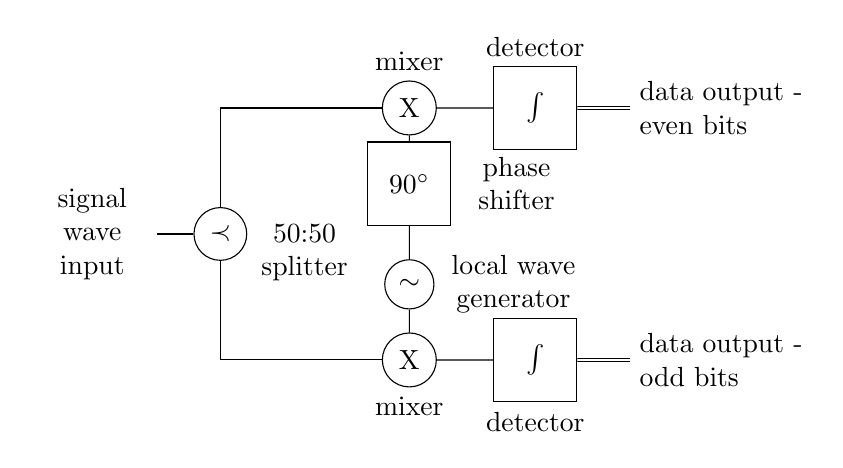
\begin{tikzpicture}[scale=0.8]
    \path
    (0,-0.8) node[circle, draw=black] (lo) {$\sim$}
    (0,0.8) node[Gate] (p90) {$90^\circ$}
    (0,2) node[circle, draw=black] (ta) {X}
    (0,-2) node[circle, draw=black] (ba) {X}
    (2,2) node[Gate] (tm) {$\int$}
    (2,-2) node[Gate] (bm) {$\int$}
    (-3,0) node[circle, draw=black] (split) {$\prec$}
     (-4,0) node[text width=40, align=center, anchor=east] (input) {signal wave input};
    \path (3.5,2) node[text width=60, align=left, anchor=west] (even) {data output - even bits}
    (3.5,-2) node [text width=60, align=left, anchor=west] (odd) {data output - odd bits};

    \draw (lo.east) node[text width=50, align=center, anchor=west] {local wave generator};
    \draw (p90.east) node[text width=40, align=center, anchor=west] {phase shifter};
    \draw (tm.north) node[anchor=south] {detector};
    \draw (bm.south) node[anchor=north] {detector};
    \draw (ta.north) node[anchor=south] {mixer};
    \draw (ba.south) node[anchor=north] {mixer};
    \draw (bm) -- (ba) -- (lo) -- (p90) -- (ta) -- (tm);
    \draw[double] (even) -- (tm);
    \draw[double] (odd) -- (bm);

    \draw (ba) -| (split)  |- (ta);
    \draw (split.south east) node[text width=40, align=center, anchor=west] {50:50 splitter};
    \draw (split) -- (input);    
\end{tikzpicture}
    \caption{Symmetric QPSK demodulator.}
\end{figure}

\section{Polarization modulation}
For an electromagnetic wave, the vibration of its electric field is always perpendicular to its direction of propagation, as shown in Fig. \ref{Polarization}, just like the vibration of a string. The polarization can be characterized by the angle of the vibration $\theta$ as shown in Fig. \ref{PolarM}.

\begin{figure}[h]\label{Polarization}
\includegraphics[width=10cm]{pic/Polarization-of-Light.jpg}
\caption{Polarization}
\end{figure}

In modern optical fiber and free space communication, polarization modulation\index{polarization modulation} is used in combination with phase modulation. The digital scheme, dual-polarization quadrature phase shift keying\index{dual-polarization quadrature phase shift keying} (DP-QPSK\index{DP-QPSK}), in particular, is mostly used. Optical fiber communication is the backbone of all our daily communication on early. Free-space communication, on the other hand, is mostly used in earth-satellite and satellite- satellite communication. As more and more communication satellites are being launched into space by companies such as Starlink, free-space communication is becoming more and more important.

So far, quantum communication experiments have all been conducted in free space or through optical fibers. Information has all been represented in qubits by a combination of phase modulation and polarization modulation of a wave. In Appendix \ref{A-qubit}, we show that the modulation in all types of qubit constructs is a combination of phase modulation plus modulation of a wave parameter mathematically equivalent to polarization modulation.

As with phase modulation, any two waves whose polarizations are orthogonal to each other have zero overlap and are least prone to noise and errors during measurement. We usually use $\theta$ to note the angle of the polarization relative to the horizontal plane. $\theta$ is between $0^\circ$ and $180^\circ$. As with phase, another significance of two waves of orthogonal polarizations is that their mixture can produce a wave of any polarization. For example, mixing $cos\theta$ portion of the wave with horizontal polarization and $sin\theta$ portion of the wave of vertical polarization produces a wave of phase $\phi$. 

\subsection{Graphical depiction}
We can replace $\phi$ with $\theta$ to draw a 2-D constellation diagram to depict polarization modulation intuitively. Fig. \ref{DP-QPSK} shows the modulation points of a double polarization modulation scheme. But how can we graphically depict a modulation combining two parameters, $\theta$ and $\phi$? We can use the spherical coordinate $(A, \theta, \phi)$ to show the modulation points as shown in Fig. \ref{DP-QPSK} for DP-QPSK.

Engineers usually do not use diagrams to depict modulations involving parameters other than phase and amplitude. But physicists use a Bloch diagram to show the spin and phase of an electron wave. Spin is the polarization of an electron wave. In a Bloch diagram, the amplitude $A$ is always 1.

\begin{figure}[h]
\begin{tikzpicture}
    \draw[->] (-3.5,0) -- (3.5, 0);
    \draw[->] (0,-3.5) -- (0,3.5);
    \draw[dotted, red] (0,0) circle(3cm);
    \draw[red, fill] (30:3) circle(0.05cm);
    \draw[dashed] (1,0) arc (0:30:1) node[right, pos=0.6]{$\theta$};
    \draw[dashed] (30:0.1) -- (30:2.9) node[pos=0.5, rotate = 30, above] {A=1};
\end{tikzpicture}
\caption{Polarization modulation}
\label{PolarM}
\end{figure}

%\node [constellation_cir] at (0,0) {};
\begin{figure}[h]\label{DP-QPSK}
\tdplotsetmaincoords{75}{110}
\pgfmathsetmacro{\h}{3.53}
\pgfmathsetmacro{\hn}{-3.53}
\pgfmathsetmacro{\r}{5}
\pgfmathsetmacro{\rn}{-5}
\begin{tikzpicture}[tdplot_main_coords]
\tdplotsetcoord{P1}{\r}{45}{45}
\tdplotsetcoord{P2}{\r}{-45}{45}
\tdplotsetcoord{P3}{\r}{45}{-45}
\tdplotsetcoord{P4}{\r}{-45}{-45}

\tdplotsetcoord{P5}{\r}{135}{45}
\tdplotsetcoord{P6}{\r}{-135}{45}
\tdplotsetcoord{P7}{\r}{135}{-45}
\tdplotsetcoord{P8}{\r}{-135}{-45}

\shade[ball color=gray, tdplot_screen_coords, opacity=0.10] (0,0,0) circle [radius=\r];

\tdplotdrawarc[gray]{(0,0,0)}{5}{-75}{105}{}; \tdplotdrawarc[dashed, gray]{(0,0,0)}{\r}{105}{285}{};
\tdplotsetthetaplanecoords{90}
\tdplotdrawarc[tdplot_rotated_coords, gray!70]{(0,0,0)}{\r}{-38}{157}{};
\tdplotdrawarc[tdplot_rotated_coords,dashed, gray]{(0,0,0)}{\r}{150}{335}{};

\draw[gray!50] (\rn,0,0) -- (\r,0,0);
\draw[gray!55] (0,\rn,0) -- (0,\r,0);
\draw[gray!60] (0,0,\rn) -- (0,0,\r);

\draw[thick, -Stealth] (\r,0,0) -- (9,0,0) node[black, left] {$x$};
\draw[thick, -Stealth] (0,\r,0) -- (0,7,0) node[black, right] {$y$};
\draw[thick, -Stealth] (0,0,\r) -- (0,0,7) node[black, left] {$z$};

\fill[red] (P1) circle (0.1); \fill[red!50] (P2) circle (0.1);
\fill[red] (P3) circle (0.1); \fill[red!50] (P4) circle (0.1);
\fill[red] (P5) circle (0.1); \fill[red!50] (P6) circle (0.1);
\fill[red] (P7) circle (0.1); \fill[red!50] (P8) circle (0.1);
\node[above] at (P1) {$(\frac \pi 4, \frac \pi 4)$};
\node[below] at (P2) {$(\frac \pi 4, \frac {5\pi} 4)$};
\node[above right] at (P4) {$(\frac \pi 4, \frac {3\pi} 4)$};
\node[below left] at (P3) {$(\frac \pi 4, \frac {7\pi} 4)$};
\node[above] at (P5) {$(\frac {3\pi} 4, \frac \pi 4)$};
\node[above] at (P6) {$(\frac {3\pi} 4, \frac {5\pi} 4)$};
\node[above right] at (P8) {$(\frac {3\pi} 4, \frac {3\pi} 4)$};
\node[below left] at (P7) {$(\frac {3\pi} 4, \frac {7\pi} 4$};

\draw[dashed, black!70] (0,0,0) -- (2.5, 2.5, 0) -- (P1); \draw[dashed, red!60] (0,0,0) -- (P1); %cycle;
\draw[dashed, red!30] (0,0,\h) circle (\h);
\draw[dashed, red!30] (0,0,\hn) circle (\h);

\tdplotsetthetaplanecoords{45}
\tdplotdrawarc[tdplot_rotated_coords, -Latex]{(0,0,0)}{2}{0}{45}{anchor=north east}{$\theta$}

\draw [thick, -Latex, canvas is xy plane at z=0] (2,0) arc [start angle=0, end angle=45, radius=2];
\node at (2,0.5,-0.3) {$\phi$};

\end{tikzpicture}
\caption{Modulation points of DP-QPSK}
\end{figure}

\subsection{Algebraic notation}
As we described in the previous section, the modulation point of a wave can be noted using the spherical coordinate $(A, \theta, \phi)$, which relates directly to the physical parameters of the carrier wave. Another notation is the complex Cartesian coordinate $(Acos\theta, Ae^{i\phi} sin\theta )$. And we can consider $Acos\theta$ representing the horizontal polarization component of the wave and $Ae^{i\phi} sin\theta$ representing the vertical component. Then $\phi$ is the phase of the vertical component relative to the horizontal component. If we consider both of their phases relative to a certain reference wave, we can use a complex Cartesian coordinate $(Ae^{i\phi_0} cos\theta, Ae^{i\phi_1} sin\theta )$ to represent the two components of the wave. Physicists like to use a complex number pair $(x_0, x_1)$, where $x_0 = Ae^{i\phi_0} cos\theta$ and $x_1 = Ae^{i\phi_1} sin\theta$, to note the wave.

\subsection{DP-QPSK demodulation}
\begin{figure}\label{Demodulator-DP-QPSK}
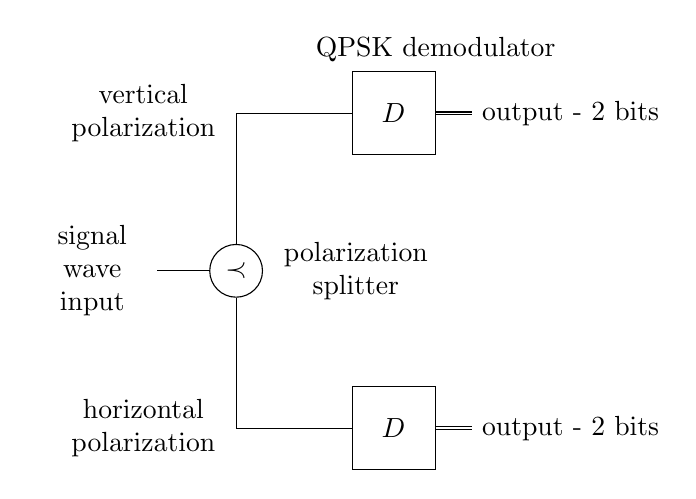
\begin{tikzpicture}[scale=1]
    \path
    (-3,0) node[text width=40, align=center, anchor=east] (input) {signal wave input}
    (-2,0) node[circle, draw=black] (split) {$\prec$}
    (0,2) node[Gate] (tsp) {$D$}
    (0,-2) node[Gate] (bsp) {$D$};
     
    \path 
    (-2,2) node [text width=60, align=center, anchor=east] (V) {vertical polarization}
    (-2,-2) node [text width=60, align=center, anchor=east] (H) {horizontal polarization}
    (1,2) node [anchor=west] (bit01) {output - 2 bits}
    (1,-2) node [anchor=west] (bit00) {output - 2 bits};

    \draw[double] (tsp) -- (bit01);
    \draw[double] (bsp) -- (bit00);
    
    \draw (input) -- (split) |- (tsp);
    \draw (split) |- (bsp);
    \draw (split.east) node[text width=60, align=center, anchor=west] {polarization splitter};
    \draw (tsp.north east) node[anchor=south] {QPSK demodulator};
\end{tikzpicture}
    \caption{DP-QPSK demodulator}
\end{figure}

\chapter{Quantum information of a single qubit}\label{c-qinfo}
In the previous chapter, we studied how information can be represented or carried by waves. All that applies to qubits for quantum computing and communication. However, the fact that the wave in each qubit has only one quantum of energy or mass imposes fundamental limitations on the measurement of the qubit or, in other words, information extraction from the qubit. This chapter studies how this limitation determines the modulation points can be used or best used by qubits. Of course, qubits with only one quantum of energy or mass in each are even more vulnerable to noise and errors, which are the main factors determining the modulation points in conventional communication channels. But qubit noise and errors are the subject of quantum error correction and are not a subject in this chapter.

\section{Measurable waves}
Measuring a qubit is an attempt to read the information carried by the wave into a conventional memory device, which uses electrical voltage or current to represent information. As shown in Fig. \ref{Demodulator-DP2}, a DP-QPSK demodulator for optical fiber communication splits the received input wave into four equal but orthogonal waves to be resonated with the four equal portions of a locally generated wave. Four photodetectors convert the photo energy of the four resonances to electrical signal currents.

To measure a qubit, the wave is split into two waves of orthogonal polarizations as shown in Fig. \ref{Demodulator-QP} before bringing them to resonate with the electrons in each of the single-photon detectors in the $M$ boxes. We do not have a locally generated wave. The equal but orthogonally polarized waves are fed directly into the photodetectors to resonate with the electrons.

Because we have no knowledge of the phases of the electron waves, we cannot measure the phase $phi$ of the input qubit wave. Further, because the qubit has only one photon and only one of the photodetectors produces photo-current, we cannot measure the polarization $\theta$ of the qubit wave either unless we know in advance that its polarization is either zero or $90$ degree. This is the fundamental limit of qubit measurement: only up to one bit of information can be extracted from a qubit.

\begin{figure}\label{Demodulator-QP}
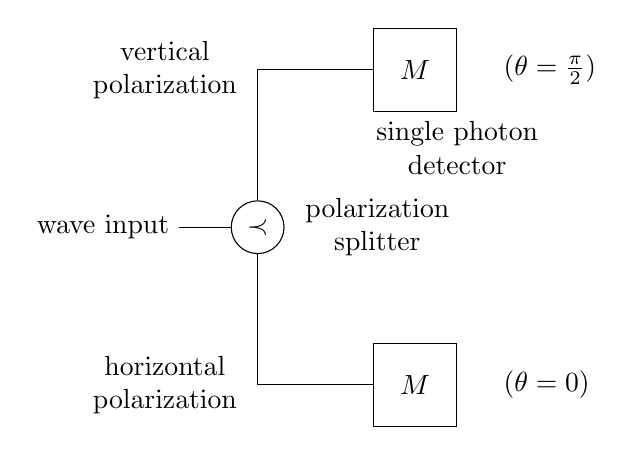
\begin{tikzpicture}[scale=1]
    \path
    (-3,0) node[anchor=east] (input) {wave input}
    (-2,0) node[circle, draw=black] (split) {$\prec$}
    (0,2) node[Gate] (tsp) {$M$}
    (0,-2) node[Gate] (bsp) {$M$};
     
    \path 
    (-2,2) node [text width=60, align=center, anchor=east] (V) {vertical polarization}
    (-2,-2) node [text width=60, align=center, anchor=east] (H) {horizontal polarization}
    (1,2) node [anchor=west] (bit01) {$(\theta=\frac \pi 2)$}
    (1,-2) node [anchor=west] (bit00) {$(\theta=0)$};

    \draw (input) -- (split) |- (tsp);
    \draw (split) |- (bsp);
    \draw (split.east) node[text width=60, align=center, anchor=west] {polarization splitter};
    \draw (tsp.south east) node[text width=60, align=center, anchor=north] {single photon detector};
\end{tikzpicture}
    \caption{Measuring a polarization qubit}
\end{figure}

\section{Modulation point notation}
From the previous chapter, we understand that information carried by a wave in a qubit can be described by a pair of real numbers $(\theta, \phi)$ in the polar coordinate or a pair of complex numbers $(x_0, x_1)$ where $|x_0|^2 + |x_1|^2 = 1$. Polar coordinates are best for visualizing modulation points graphically, which all fall on the sphere in Fig. \ref{DP-QPSK}. The sphere is called the Block sphere by physicists.

\subsection{Tensor notation}
The complex number pair notation $(x_0, x_1)$ is easier to use when studying a quantum gate transforming a qubit from one modulation point to another, say $(x'_0, x'_1)$. Physicists usually use the transpose of the complex coordinates, which are tensors. So, we can write a transformation as a matrix multiplying the transposed tensor of the original coordinate:
\begin{equation}
    \begin{pmatrix}
    x'_0 \\
    x'_1
\end{pmatrix}
=
    \begin{pmatrix}
    t_{0,0} & t_{0,1} \\
    t_{1,0} & t_{1,1} 
\end{pmatrix}
    \begin{pmatrix}
    x_0 \\
    x_1
\end{pmatrix}.
\end{equation}
Here, the matrix
\begin{equation}\label{e-T}
T
=
    \begin{pmatrix}
    t_{0,0} & t_{0,1} \\
    t_{1,0} & t_{1,1} 
\end{pmatrix}
\end{equation}
is the transformation matrix representing the gate.

\subsection{Ket notation}
Physicists favor what is called the ket notation, which actually is a vector notation. The unit vectors $\hat x_0$ and $\hat x_1$ are written as $\keta{0}$ and $\keta{1}$. Therefore, a modulation point can be written as $cos{\theta} \keta{0} + e^{i \phi} sin{\theta} \keta{1}$ or $x_0 \keta{0} + x_1 \keta{1}$. Here, the "$+$" is mathematically a vector addition. Physicists interpret the "$+$" as superposition -- coherent mixing or addition of two waves.

The ket notation provides physicists with a brief notation along with associated physical meaning. In the ket notation, transformations of quantum gates are written as abstract operators. So, the ket notation is best for theoretical derivation but not for numerical calculation. Its advantage is also in describing a circuit of $n$-qubits, as we will see soon.

\section{Single qubit transformation and gates}\label{Sec-Plus}
Throughout this book, we can find that the mostly used modulation points of a single qubit are the $\keta{0}$, $\keta{1}$, $\keta{+}$ and $\keta{-}$ shown in Fig. \ref{qQPSK}.

\begin{figure}[h]\label{qQPSK}
%\includegraphics[width=6cm]{pic/qqpsk.jpg}
\begin{tikzpicture}
    \draw[->] (-3.5,0) -- (3.5, 0);
    \draw[->] (0,-3.5) -- (0,3.5);
    \draw[dashed] (2.5,2.5) -- (0,0);
    \draw[dashed] (0,0) -- (2.5,-2.5);
    \draw[dotted, red] (0,0) circle(3cm);
    \draw[red, fill] (3,0) circle(0.05cm) node[below right] {\ket{0} - 00};
    \draw[red, fill] (0,3) circle(0.05cm) node[above right] {\ket{1} - 01};
    \draw[red, fill] (2.12,2.12) circle(0.05cm) node[right] {\ket{+} - 11};
    \draw[red, fill] (2.12,-2.12) circle(0.05cm) node[below] {\ket{-} - 10};
    \draw[dashed] (1,0) arc (0:45:1) node[right, pos=0.6]{$\theta=\pi/4$};
\end{tikzpicture}
\caption{Constenlation diagram of quantum $\theta$ shift keying}
\end{figure}

\subsection{$X$ gate}
Quantum algorithms always assume a qubit is initiated at the $\keta{0}$ point. Even the measurable $\keta{1}$ point is transformed from it by an $X$ gate\index{X gate}.
In a $\theta$ constellation diagram, an $X$ gate swaps the $x$ and $y$ axes or is a 2-D reflection across the $45^\circ$ line. In vector notation, the transformation of an $X$ gate is expressed as a matrix,
\begin{equation}
    X = \begin{pmatrix}
        0 & 1 \\
        1 & 0
    \end{pmatrix}.
\end{equation}
In a circuit diagram, an $X$ gate is the letter $X$ in a box. Therefore, the transformation from $\keta{0}$ to $\keta{1}$ can be drawn as
\begin{figure}[h]\label{X1}
\begin{quantikz}
    \lstick{\ket{0}} & \gate{X} & \qw \rstick{\ket{1}}
\end{quantikz}
\caption{Use X gate to produce a $\keta{1}$ wave.}
\end{figure}

An $X$ gate can also be represented as $\bigoplus$. But in this book, we do not use this notation.

Beside the $X$ gate, literatures also talk about Pauli $Y$ and $Z$ gates, which transform a qubit according to the Pauli matrices\index{Pauli matrices}:
\begin{equation}
\begin{array}{rl}
    Y & = \sigma_y = \begin{pmatrix}
        0 & -i \\
        i & 0
    \end{pmatrix} \\
    Z & = \sigma_z = \begin{pmatrix}
        1 & 0 \\
        0 & -1
    \end{pmatrix}
\end{array}
\end{equation}

\subsection{Hadamard gate}
The $\keta{+}$ wave can be view as the $\keta{0}$ wave subjected to a 45-degree polarization rotation and can also be viewed as a superposition state of the $\keta{0}$ and $\keta{1}$ waves. In a circuit, it is transformed from a $\keta{0}$ by a Hadamard gate as shown in Fig. \ref{H+}. A Hadamard gate reflects all the points on the $\theta$ constellation diagram across the 22.5 degree axis shown in Fig. \ref{qQPSK}. Its circuit symbol is the letter "H" enclosed in a square. Reflecting a $\keta{0}$ qubit across the axis obvious becomes a qubit of 45-degree polarization -- the $\keta{+}$ state. And reflecting the $\keta{1}$ qubit across the axis becomes a qubit of -45 degree polarization -- the $\keta{-}$ state.
\begin{figure}[h]\label{H+}
\begin{quantikz}
    \lstick{\ket{0}} & \gate{H} & \qw \rstick{\ket{+}}
\end{quantikz}
\caption{Use H gate to produce $\keta{+}$ wave.}
\end{figure}

The $\keta{-}$ wave can be view as the $\keta{0}$ wave subjected to a -45-degree polarization rotation and can also be viewed a superposition wave of the $\keta{0}$ and the $\keta{1}$ waves with 180-degree phase shift. In a circuit, it is transformed from a $\keta{1}$ by a Hadamard gate as shown in Fig. \ref{H-}.
\begin{figure}[h]
\begin{quantikz}
    \lstick{\ket{0}} & \gate{X} & \gate{H} & \qw \rstick{\ket{-}}
\end{quantikz}
\caption{Use H gate to produce $\keta{-}$ wave.}
\label{H-}
\end{figure}

\subsection{Wave characteristics for qubit modulation}
\begin{table}[]
\caption{Wave characteristics for qubit modulation}
\label{modulation-characteristics}
\begin{tabular}{lll}
Wave parameters &Represented numbers &Qubit design   \\
Amplitude & Number of qubits 1, 2, ... & all qubits \\
Phase & $\phi \in (-\pi /2, \pi /2] $& all qubits \\
Frequency & $\theta \in (-\pi /2, \pi /2]$ & SC-IBM, Google; trapped ion - IonQ \\
Mode & $\theta \in (-\pi /2, \pi /2]$ & Xanadu, PsiQuantum \\
Polarization & $\theta \in (-\pi /2, \pi /2]$ & USTC \\
Spin & $\theta \in (-\pi /2, \pi /2]$ & 
\end{tabular}
\end{table}

\section{BB84 protocol}
Charles Bennett and Gilles Brassard proposed in 1984 a quantum encryption protocol\cite{BB84}. But it is not practical for encryption. It is more practical if used for cipher key distribution.

\subsection{BB84 as an encryption protocol}
By tradition, all communication encryption protocols are narrated as the scenario that Alice wants to transmit a series of data bits to Bob but fears Eve may eavesdrop the communication channel\cite{Schneier}. The protocol assumes:
- Alice has a series of data bits to be encrypted; she also has another series of encryption key bits, which are random;
- Bob has the same series of key bits, but expects to receive the data bits securely.

In each time slot, the protocol goes through the following steps to transmit one data bit:
- Alice takes one bit from each series to form a 2-bit symbol -- the first bit from the data series and the second from the key series;
- This step can be stated in two versions: from a physicist's perspective, Alice maps the data bit to the $\beta{0}$, $\beta{1}$ modulation points; if the key bit is 1, she rotates the polarization of the modulation point by $45^\circ$; from an engineer's perspective, Alice maps the 2-bit symbol, 00, 01, 10 or 11, to the $\beta{0}$, $\beta{1}$, $\beta{-}$ or $\beta{+}$ modulation point;
- Alice sends the qubit to Bob;
- There can be two versions to state how Bob recover the data bit: from a physicist's perspective, Bob rotates the wave's polarization by $-45^\circ$ if the key bit is 1; from an engineer's perspective, the key bit value determines whether to apply a Hadamard gate as shown in the circuit diagram \ref{BB84}.

\begin{figure}[h]
\label{BB84}
\begin{quantikz} %[wire types={q,c}]
    \lstick{Alice' data bits}  & \cwbend{1} \\
    \lstick{\ket{0}} & \gate{X} & \gate{H} &\qw & \qw & \gate{H} & \meter{} &\cw \rstick{data output} \\
    \lstick{Alice' key bits}  & \cw & \cwbend{-1} &\slice{Eve} & & \cwbend{-1} & \cw \rstick{Bob's key bits}
\end{quantikz}
\caption{BB84 circuit}
\end{figure}

Performance
Qubits per channel: one qubit
Channel capacity: one data bit per transmission time slot
Channel efficiency: 50\%.

From a cryptographer perspective, the protocol has two problems:
- it cannot tell whether a symbol received is a re-transmitted from Eve;
- it is an one-time pad encryption -- each key bit is used for only one data bit -- and is not practical for real encryption.
the following sections address these problems.

\subsection{Adding authentication to BB84 protocol}
A quantum protocol such as BB84 is immune to wire-tapping, but like other protocols, it is vulnerable to attacks if Eve intercepts the qubits from Alice and sends Bob qubits produced by herself. Not part of the BB84 protocol, the standard approach to detect such attacks is to add $m$ authentication bits, which are bits known to both Alice and Bob in advance, to every $n$ data bits: $a_1 a_2 ... a_m d_1 d_2 ...d_n$. If Bob finds the authentication bits not being what he expects, he discards the block of $m+n$ bits.

\subsection{Key distribution}
All OTP protocols such as BB84 are theoretically beautiful but are not practical because they require encryption keys to be equal lengths as the data messages. It is a chicken and egg dilemma: how does Alice shares or distributes the series of secret key bits to Bob at the first place? Conventional public key exchange protocols are the current solutions. But they have many problems. They require expansive computation and may be broken by the power of quantum computing.

BB84 protocol and the quantum protocols following it do not depend on expansive computation. They recognize the fact that keys are random numbers. And key distribution or sharing can afford to lose some candidate key bits and does not require all candidate key bits being accepted by Bob. Alice can distribute all the candidate key bits to Bob. And Bob and Alice only need to agree on which of the candidate bits are "good" to use.

BB84 modifies the above protocol for key distribution in the following way:
- Alice generates two blocks of random bits of equal length with one block being the data bits -- or candidate key bits -- and another as the "encryption" key bits.
- Alice pairs the bits 00, 01, 10, or 11, and send it to Bob in the quantum channel (the qubit) mapped to the modulation points shown \ref{qQPSK}. Anyone who measures the qubit and gets a result of "0" cannot distinguish the actual code point is "00" or "10". So the original data is encrypted.
- Bob does not have the "encryption" key bits that Alice uses but has a series of key bits out of his random generation. And Bob demodulates each received qubit using his key bit and obtain his data bits.
- Alice and Bob then use a conventional communication channel to compare their corresponding key bits. If they agree, Alice and Bob keeps the candidate data bit. Otherwise, the candidate bit is discarded.

With many of the original data bits from Alice being discarded, what is good of BB84? The good part is that the kept data bits can be used as the key for future encryption. Therefore, BB84 is considered a quantum key distribution protocol. The quantum channel guarantees that it cannot be tapped. But it cannot prevent an eavesdropper Eve from intercepting the qubits in the channel. Eve may intercept the qubits without sending anything to Bob and may also attempt to reproduce the qubit to send to Bob. Because of the no-cloning theorem, Eve cannot reproduce the qubit to disguise the interception. So, key distribution with BB84 guarantees keys' confidentiality and integrity although the rate of key transmission may suffer from interception.

\chapter{Quantum information of multiple qubits}\label{c-n-qubit}
The smallest information-carrying unit of a conventional computer is a bit stored in a pair of transistors. From there, 8, 16, 32, or 64 bits are used together as units like a byte, INT16, INT32, or FLOAT for processing. All these units are of fixed sizes. The advantage of graphics processing units (GPUs)\index{GPU} lies in their capability to process in parallel such units of multiple bits.

In a communication channel, the smallest information carrier is called a carrier or sub-carrier, which is a wave at a particular frequency. To increase capacity, several sub-carriers at different frequencies are combined in a channel to transmit in the same medium e.g. radio airway or optical fiber. The sub-carriers must have frequencies sufficiently separated so that the receiver can distinguish them. How many sub-carriers can be squeezed in the same channel and how to combine them so that the sub-carriers can be maximally distinguished at the receiver end is an area of study called multiplexing by communication engineers.

Multiplexing qubits may serve two purposes
- combining multiple qubits into a unit for parallel processing by quantum gates or
- transfer the $n$-bit result in one qubit into $n$ qubits so that $n$ bits can be retrieved by measurement.
When multiplexing, the wave in each qubit remains physically separated from the others. But their phases are synchronized so that they can be processed by a quantum gate as one wave. This chapter studies multiplexing of the waves of multiple qubits.

\section{Measurable waves}
In the previous chapter, we label the measurable waves of a qubit with $0$ and $1$ and note the corresponding wave functions as $\keta{s}$, where $s=0, 1$. Naturally, we label the measurable waves of $n$ qubits with $(s_1, s_2, ..., s_n)$ where $i=1, 2, ...n$ and note their wave functions as
\begin{equation}\label{e-nqubit}
    \keta{s_1, s_2, ..., s_n} or
    \keta{s_1} \keta{s_2} ... \keta{s_n}
\end{equation}
where $s_i = 0, 1$ and $i=1, 2, ..., n$.

Similar to the wave functions of a single qubit, the wave functions in Eq. \ref{e-nqubit} are the base vectors of a $2^n$-dimensional Hilbert space. $n$-qubit modulation points are superpositions of the bases:
\begin{equation}
    \keta{w} = \sum_{s_1=0,0; s_2=0,1; ...; s_n=0,1} x_{s_1, s_2, ..., s_n} \keta{s_1, s_2, ..., s_n}.
\end{equation}

\section{2-qubit transformation and gates}

\subsection{Bell states}
Like in the cases of one qubit and QPSK, we can also use superpositions of the above base waves to come up with a new set of base waves:
\begin{equation}
\begin{array}{rl}
    \keta{B_{00}} =& \frac 1 {\sqrt 2} (\keta{0}\keta{0}+\keta{1}\keta{1}),\\
    \keta{B_{01}} =& \frac 1 {\sqrt 2} (\keta{0}\keta{1}+\keta{1}\keta{0}),\\
    \keta{B_{10}} =& \frac 1 {\sqrt 2} (\keta{0}\keta{0}-\keta{1}\keta{1}),\\
    \keta{B_{11}} =& \frac 1 {\sqrt 2} (\keta{0}\keta{1}-\keta{1}\keta{0}).
\end{array}
\end{equation}
The second set of base waves can be considered 45 degree rotated from the first set. Physicists call them Bell state waves and use the funny symbols to note them. They are in the form $cos\theta |b_i> + sin\theta e^{i\phi} |b_j>$. They are no longer separable waves.

We can use 8 waves from the 2 sets of bases to represent numbers of 3 bits as shown in Fig. \ref{2qQPSK}.
\begin{figure}\label{2qQPSK}
\begin{tikzpicture}
    \draw[->] (-3.5,0) -- (3.5, 0);
    \draw[->] (0,-3.5) -- (0,3.5);
    \draw[dashed] (2.5,2.5) -- (-2.5,-2.5);
    \draw[dashed] (-2.5,2.5) -- (2.5,-2.5);
    \draw[dotted, red] (0,0) circle(3cm);
    \draw[red, fill] (0:3) circle(0.05cm) node[above right] {$b_{00}$};
    \draw[red, fill] (90:3) circle(0.05cm) node[above right] {$b_{11}$};
    \draw[red, fill] (45:3) circle(0.05cm) node[above left] {$B_{00}$};
    \draw[red, fill] (-45:3) circle(0.05cm) node[above right] {$B_{10}$};
\end{tikzpicture}
\begin{tikzpicture}
    \draw[->] (-3.5,0) -- (3.5, 0);
    \draw[->] (0,-3.5) -- (0,3.5);
    \draw[dashed] (2.5,2.5) -- (-2.5,-2.5);
    \draw[dashed] (-2.5,2.5) -- (2.5,-2.5);
    \draw[dotted, red] (0,0) circle(3cm);
    \draw[red, fill] (90:3) circle(0.05cm) node[below left] {$b_{01}$};
    \draw[red, fill] (0:3) circle(0.05cm) node[above right] {$b_{10}$};
    \draw[red, fill] (45:3) circle(0.05cm) node[below right] {$B_{01}$};
    \draw[red, fill] (-45:2) circle(0.05cm) node[below left] {$B_{11}$};
\end{tikzpicture}
    \caption{2 qubit base states and Bell states}
\end{figure}

\subsection{Producing Bell states}
\begin{figure}[h]
\begin{quantikz}
    \lstick{\ket{+}}  & \ctrl{1} & \qw \rstick[2]{\ket{\Phi^+}} \\
    \lstick{\ket{0}} & \gate{X} &\qw 
\end{quantikz}
\caption{Producing Bell states}
\label{BS}
\end{figure}
Changing the input waves from $\keta{+}$ to $\keta{-}$ or from $\keta{0}$ to $\keta{1}$, we can obtain the other Bell states.


\section{Quantum gates for information processing}
Qubits are memory devices or communication channels. Quantum gates are processing devices that can change the modulation of $\theta$ and phase $\phi$. As desired by the algorithms, the gates are concatenated or connected into circuits. Other than measuring gates, no gate changes the amplitude of the qubits in a circuit. Therefore, all gate transformations are unitary and can be expressed as
\begin{equation}
G=
    \begin{pmatrix}
        cos\delta \theta & -e^{i\delta \lambda} sin\delta \theta \\
        e^{i \delta \phi} sin\delta \theta & e^{i \delta \phi+ \delta \lambda} cos\theta 
    \end{pmatrix} or
G=   \begin{pmatrix}
        g_{00} & g_{01} \\
        g_{10} & g_{11} 
    \end{pmatrix}
\end{equation}
where $G^\dagger = G$

\subsection{Control gates}
Assume $f(x)$ is a binary function mapping $x \in {0,1}$ to ${0,1}$. The control-f gate takes input waves $\keta{x}\keta{y}$, where $x$ and $y$ are either 0 or 1, and produce the output waves as shown below.
\begin{figure}[h]
\begin{quantikz}
    \lstick{\ket{x}}  & \ctrl{1}  & \qw \rstick{\ket{x}} \\
    \lstick{\ket{y}} & \gate{f} &\qw \rstick{\ket{y\bigoplus f(x)}}
\end{quantikz}
\caption{Control-f gate}
\label{c-f}
\end{figure}
A particularly important type of control gates is the control-NOT or C-NOT gates, in which the $f$ is the Pauli $X$. A C-NOT gate is best described in vector notation as matrix
\begin{equation}
    \begin{pmatrix}
1 & 0 & 0 &0 \\
0 & 1 & 0 &0 \\
0 & 0 & 0 & 1 \\
0 & 0 & 1 & 0
\end{pmatrix}
\end{equation}

\section{Circuit diagrams}
A algorithm or protocol is always depicted by a circuit diagram or series of matrix calculations. In circuit diagram, a qubit is shown as a line, and a gate as a rectangle.

\chapter{Quantum Communication Protocols}\label{c-comm}
Encryption is used in everyday Internet communication. Encryption conceals the credit card numbers and passwords, which we send to the e-commerce websites. But we don't know whether or not the communication is being tapped for eavesdropping. In fact, our communications with international parties are routinely tapped and monitored by various national security agencies.

The significant use of quantum technology in communication is its anti-eavesdropping feature. If a communication carrier is a qubit, which has a wave of only one quantum, partial tapping is impossible. Eavesdropping can only be accomplished by intercepting the qubit. Further, the eavesdropper may attempt to clone the intercepted qubit and transmit the clone to the receiver to avoid detection. In this chapter, we discuss how quantum communication protocols can be designed to overcome the security challenges.

\section{Superdense coding}
Superdense coding is also called dense coding. It takes advantage of the fact that the waves of two entangled qubits are aligned to be one wave so that we can use the parameter $\delta$ to carry information. The appearance is that two bits of information are carried by one qubit. But the information is actually encoded in two qubits.

As shown in the circuit diagram Fig. \ref{denseCoding}, the operation first entangles the qubit in Alice' possession remotely with the one possessed by Bob. The state of the entangled qubits is $\keta{B_00}$. Alice modulates her qubit with the $X$ and $Z$ gates according to two input bits before passing the qubit to Bob. The resulting state of the qubits changes among the Bell states as shown in Table \ref{t-DenseCoding}. Bob then dde-entangle the two qubits before measuring the qubits recover the two-bits of information.

This protocol for encrypting the 2nd bits.

\begin{table}[]
\label{t-DenseCoding}
\caption{Modulate one qubit in an entanglement to encode 2 bits}
\centering
\begin{tabular}{lll}
Digital input & Operation & Result   \\
00 & None   & $B_00$ \\
01 & X   & $B_01 $  \\
10 & Z   & $B_10 $ \\
11 & XZ  & $B_11 $ 
\end{tabular}
\end{table}

\subsection{Circuit diagram}
\begin{figure}[h]\label{denseCoding}
\begin{quantikz}%[slice all, slice style={shorten <=8mm}, slice label style = {yshift=-38mm} ]
    & & &\lstick{Alice' 2nd bit}  & \cwbend{2} \\
    & & \lstick{1st bit}  & \cwbend{1} \\
    \lstick{Alice' \ket{0}} & \gate{H} &\ctrl{1} & \gate{X} & \gate{Z} &\ctrl{1} & \gate{H} & \meter{} &\cw \rstick{Bob's 1st bit} \\
    \lstick{Bob's \ket{0}} & \qw      & \targ{} \slice[style={shorten <=12mm}, label style={yshift=-38mm}]{\ket{B_00}} & \qw \slice[style={shorten <=12mm}, label style={yshift=-38mm}]{\ket{B_01}} & \qw \slice[style={shorten <=12mm}, label style={yshift=-38mm}]{\ket{B_11}} & \targ{} & \qw & \meter{} & \cw \rstick{Bob's 2nd bit}
\end{quantikz}
\caption{Superdense coding circuit}
\end{figure}

\section{Teleportation}
\subsection{Circuit diagram}
\begin{figure}[h]
\begin{quantikz}%[slice all, slice style={shorten <=8mm}, slice label style = {yshift=-38mm} ]
    & & \lstick{Alice' wave x\ket{0}+y\ket{1}}  & \ctrl{1} & \gate{H} & \meter{} &\cw \rstick{Alice' 1st bit} \\
    \lstick{\ket{0}} & \gate{H} &\ctrl{1} & \targ{} & \qw& \meter{} &\cw \rstick{Alice' 2nd bit} \\
    \lstick{\ket{0}} & \qw      & \targ{} \slice[style={shorten <=2mm}, label style={yshift=-38mm}]{1} & \qw & \qw & \qw \rstick{Bob's wave}
\end{quantikz}
\caption{Teleportation circuit}
\label{Teleportation}
\end{figure}

There are 3 qubits in the scheme. The 2nd and 3rd are entangled at the first stage. Alice modulates the first qubit with an analog signal encoded as $(x, y)$. The state of the qubit may be written as $x \keta{0} + y\keta{1}$. The 1st and 2nd qubits are then de-entanglement. The analog signal comes in the form of a qubit, which we call it the signal qubit. 
\begin{equation}
\begin{array}{rl}
    & (x \keta{0} + y\keta{1}) \frac 1 {\sqrt 2}(\keta{0}\keta{0}+\keta{1}\keta{1}) \\
    = & \frac 1 {\sqrt 2} (\keta{0}\keta{0}+\keta{1}\keta{1}) (x \keta{0} + y\keta{1}) \\
    +& \frac 1 {\sqrt 2} (\keta{0}\keta{0}-\keta{1}\keta{1}) (x \keta{0} - y\keta{1})  \\
    +& \frac 1 {\sqrt 2} (\keta{0}\keta{1}+\keta{1}\keta{0}) (x \keta{0} + y\keta{1}) \\
    +& \frac 1 {\sqrt 2} (\keta{0}\keta{1}-\keta{1}\keta{0}) (x \keta{0} - y\keta{1}) 
\end{array}
\end{equation}

\begin{table}[]
\caption{Modulate one qubit to encode 2 bits}
\label{TeleportationTable}
\begin{tabular}{lr}
Alice's output $d_1 d_0$ & Bob's qubit  \\
00 & $x\keta{0}+y\keta{1}$ \\
01 & $x\keta{1}+y\keta{0}$ \\
10 & $x\keta{0}-y\keta{1}$  \\
11 & $x\keta{1}-y\keta{0}$ 
\end{tabular}
\end{table}

Alice has a qubit with information S and shares a pair of qubits with Bob. The pair is one of the 4 known eigenwaves and has 2 bits of information. The total input information is therefore S+2. At the output, Alice measures the first 2 qubits against the same 4 eigenwaves and tells Bob the result, which has 2 bits of information. If no information is lost, the information in the 3rd qubit should be S.

\subsection{Quantum secure direct communication (QSDC)}
QSDC is an adaptation of quantum teleportation to key distribution. The key transmission rate is 1 bit per qubit duty cycle and is a much improvement over the BB84 protocol.

\section{Blind quantum computation (BQC)}

\chapter{Deutsch's and related algorithms}\label{c-Deutsch}

\section{Deutsch's algorithm}
A one-bit function $f$ mapping \{0,1\} -\> \{0,1\} can have 4 possible outputs, which are 2 bits of information. But the outputs belong to 2 categories, constant or balanced, which are an 1-bit information as of $f(1)+f(0)$. We can't obtain the 2-bit information using one operation but can obtain the 1-bit information if we feed the function with the $\keta{+}$ qubit:
\begin{equation}\label{DeutschF1}
\begin{array}{rl}
    U_f(\frac 1 {\sqrt 2} (\keta{0}+\keta{1}) ) = & \frac 1 {\sqrt 2} (e^{2\pi i f(0)} \keta{0}+ e^{2\pi i f(1)} \keta{1}) \\
    = & \frac 1 {\sqrt 2} e^{2\pi i f(0)} (\keta{0}+ e^{2\pi i [f(1)-f(0)]} \keta{1})
\end{array}
\end{equation}

From above derivation, we see that it takes one operation of the $F$ gate to evaluate both $f(0)$ and $f(1)$. But the result still requires two measurements, one to determine $f(0)$ and the other to determine $f(1)-f(0)$. For two measurements, we need the help of another qubits.

\subsection{Phase kick back}
\begin{figure}[h]
\begin{quantikz}
    \lstick{\ket{x=0/1}}  & \ctrl{1} & \qw \rstick{$(-1)^{f(x=0/1)}$ \ket{x=0/1}} \\
    \lstick{\ket{-}} & \gate{f} &\qw \rstick{\ket{-}} 
\end{quantikz}
\caption{Producing Bell states}
\label{phaseKick}
\end{figure}

With the help of a C-NOT gate, the 2 bits of information modulated in one qubit can be transfered to two qubits and therefore can be all extracted.

\subsection{Circuit diagram}
\begin{figure}[h]
\begin{quantikz}[scale=1.3]
    \lstick{\ket{0}} & \gate{H} & \ctrl{1} \slice{$(-1)^{f(0)}$\ket{0}+$(-1)^{f(1)}$ \ket{1} }  & \gate{H} & \meter{} &\cw \rstick{$f(1)-f(0)$} \\
    \lstick{\ket{1}} & \gate{H} & \gate{f} &\qw \rstick{\ket{-}}
\end{quantikz}
\caption{Deutsch's algorithm circuit}
\label{Deutsch}
\end{figure}

\subsection{Performance}
Processing: two quantum gates - one operation per gate; one measurement.
Memory: one qubit for the processing. But for output, two qubits are required.


\section{Mostly used modulation points}
\subsection{Measurement bases}
The measurement base waves are $\keta{x_0}\keta{x_1}\keta{x_2} ...\keta{x_{n-1}}=\prod^{n-1}_{i=0}$, where $x_i in \{0, 1\}$.

\subsection{Evenly mixed wave and Fourier bases}
Expanding on the idea of the $\keta{+}$ wave in \ref{Sec-Plus}, we can have a wave
\begin{equation}
\begin{array}{rl}
    \keta{s_0} &= \frac 1 {\sqrt{2}} (\keta[0]{0}+\keta[0]{1}) \frac 1 {\sqrt{2}} (\keta[1]{0}+\keta[1]{1})
    ... \frac 1 {\sqrt{2}} (\keta[n-1]{0}+\keta[n-1]{1}) \\
    &= \frac 1 {2^{n/2}} (\keta{b_0}+\keta{b_1}+...+\keta{b_{N-1}})
 \end{array}
\end{equation}
which is an evenly mixture of the $n$-qubit bases. But what are the orthogonal waves similar to the $\keta{-}$ of one qubit?
\begin{equation}
\begin{array}{rl}
\keta{s_k} &= \frac 1 {\sqrt{2}} ({\keta{0}}_0+{\keta{1}}_0)
    \frac 1 {\sqrt{2}} ({\keta{0}}_1+e^{\frac {k*2 \pi i} 2}{\keta{1}}_1)
    ...  \frac 1 {\sqrt{2}} ({\keta{0}}_{n-1}+e^{\frac {(n-1)*2\pi i} 2^(n-1)}{\keta{1}}_{n-1}) \\
    ... \\
    &= \frac 1 {\sqrt{N}} \prod^{n-1}_{l=0} ({\keta{0}}_l+e^{\frac {k\times l \times 2\pi i} 2^l}{\keta{1}}_l) where k=0, 1, ...N-1.
\end{array}
\end{equation}
Like the $\keta{+}$ and $\keta{-}$ waves, each of the $\{\keta{s_k}, k=0, 1, ... N-1\}$ waves is a mixture of all the base waves, but they have different orientations in the $N$ dimension Hilbert space.

\section{Design patterns}

\subsection{Producing equal superposition}

\subsection{Quantum Fourier transform}
Classical discrete Fourier transform maps a set of $N$ complex numbers ${x_0, x_1, ..., x_{N-1}}$ to another $N$ complex numbers
\begin{equation}
    y_k = \frac 1 {\sqrt{N}} \sum^{N-1}_{n=0} x_n\omega_{N}^{-nk}, k = 0, 1, 2, ..., N-1,
\end{equation}
where $w_N = e^{\frac {2\pi i} N }$. For physicists and engineers, the numbers ${y_n}$ help to reflect prominently the periodic patterns such as their frequency in $x_n$. For the same purpose, quantum Fourier transform is defined mathematically as follow but is easier to be realized by quantum gates:
\begin{equation}
    y_k = \frac 1 {\sqrt{N}} \sum^{N-1}_{n=0} x_n\omega_{N}^{xk}, k = 0, 1, 2, ..., N-1,
\end{equation}
where $x = x_0 + x_1 2^1 + x_2 2^2 + ... +x_{N-1} 2^{N-1}$. In vector notation, $F_N$ is a unitary matrix, and its $i, j$ element is
\begin{equation}
    f_{i,j} = \omega^{i.j}.
\end{equation}
This matrix is the same matrix as for the discrete Fourier transform. Therefore, quantum Fourier transform is equivalent to discrete Fourier transform.

\subsubsection{Complexity}

\subsection{Phase estimation}
\subsubsection{Complexity}

\section{Grover's algorithm}
Like the Deutsch's algorithm, the Grover's algorithm also assumes a blackbox function $f(x)$ whose variable $x$ is a $n$-bit binary variable. Its result is a single-bit value and is always 1 except for a few unknown $x=x_w$ at which $f(x_w)=-1$. The goal of the algorithm is to find the $x_w$. Lov Grover proposed in 1996 that quantum computer can solve it faster than conventional computers.

Let's assume there is one and only one solution $x_w$ as an example, and note $x_w$ as $w_{n-1}...w_i...w_1 w_0$ in binary where $w_i = 0 or 1$, and $\Vec{w} = (0, 0, ..., 1 at i=w, ..., 0)^T$ as a $2^n-1$ dimensional vector. Using conventional computers, we'd feed each of the $2^n -1$ possible numbers of $x_w$ at a time to $f$ to test whether the result equals $-1$. The worst case is that we have to do $2^n-1$ evaluations of $f(x)$ to find out $x_w$. We of course wish to explore all the possible $x_w$ at the same time. We naturally choose $\vec{S} = \frac 1 {\sqrt{2^n}} (1, 1, ...1)^T$, which is the sum of all the bases of the qubits, to feed the oracle function $f$.

We know, $\vec{S} = \vec{S} - \frac 1 {\sqrt{2^n}} \vec{w}) + \frac 1  {\sqrt{2^n}} \vec{w}$. Apparently, $\vec{S_1}  = \vec{S} - \frac 1 {\sqrt{2^n}} \vec{w}$ is a vector orthogonal to $\vec{w}$, and applying the $F$ gate to it does not change its phase. Therefore, $F(\vec{S}) = F(\vec{S_1}) + F(\frac 1  {\sqrt{2^n}} \vec{w})  = \vec{S_1} - \frac 1 {\sqrt{2^n}} \vec{w}$. We see that 
\begin{itemize}
    \item applying the $F$ gate turns vector $\vec{S}$ toward $-\vec{w}$
    \item applying the $F$ gate to $\vec{S_1}$ makes no change.
\end{itemize}
Therefore, can we apply $F$ gate $2^n$ times and turn $\vec{S}$ completely to $-\vec{w}$? But applying $F$ gate once more will change the phase of the $\vec{w}$ vector back. We need to change the sign of vector $\vec{w}$ first while preserving its angle with $\vec{S}$ before applying $F$ gate again. This can be accomplished by apply gate $U_S = 2 \vec{S}X\vec{S} -I$, which flip $\vec{w}$ around the vector $\vec{S}$. However, when implementing this flip, we need to rotate $vec{S}$ to the $\vec{0}$, do the flip, and rotate the frame back to $\vec{S}$.

\begin{figure}[h]\label{Grover}

\caption{Applying F gate}
\end{figure}

\subsection{Complexity}

\section{Simon's algorithm}
The Simon's algorithm assumes a blackbox oracle function $f(x)$ whose variable $x$ is a $n$-bit binary variable. Its results are $m$-bit values that are periodic, but the period $t$ is unknown -- $f(x+t)=(fx)$ for all $x$. How do we find the period $t$? Of course, we are tempted to play the trick again of feeding $\vec{S} = \frac 1 {\sqrt{2^n}} (1, 1, ...1)^T$ to the oracle function $f$. We have
$f(\vec{S}) = \frac 1  {\sqrt{2^n}} \sum_x f(x)$.

\subsection{Circuit diagram}
\begin{figure}[h]
\begin{quantikz}%[slice all, slice style={shorten <=8mm}, slice label style = {yshift=-38mm} ]
    & & &\lstick{Alice' 2nd bit}  & \cwbend{2} \\
    & & \lstick{1st bit}  & \cwbend{1} \\
    \lstick{\ket{0}} & \gate{H} &\ctrl{1} & \gate{Z} & \gate{X} &\ctrl{1} & \gate{H} & \meter{} &\cw \rstick{Bob's 1st bit} \\
    \lstick{\ket{0}} & \qw      & \targ{} \slice[style={shorten <=12mm}, label style={yshift=-38mm}]{BS1} & \qw \slice[style={shorten <=12mm}, label style={yshift=-38mm}]{BS2} & \qw \slice[style={shorten <=12mm}, label style={yshift=-38mm}]{BS3} & \targ{} & \qw & \meter{} & \cw \rstick{Bob's 2nd bit}
\end{quantikz}
\caption{Simon's algorithm}
\label{Simon}
\end{figure}

\subsection{Complexity}
Using conventional computer, finding the period takes $2^{n/2}$ operations.

\section{Shor's algorithm}
Much of modern day cryptography is based on the difficulty of factoring large integer numbers. Factoring 15=3x5 is easy for a person. Factoring 12140041 = 3413x3557 is impossibly hard although it is not difficult for modern day computers. Almost all Internet connections from our mobile phones and computers are based on AES, which is a private key encryption algorithm, and RSA or DH algorithms for key exchange.

For a positive integer $M$, how can we find out whether it has factors? A naive approach is to iterate over
$a=2, 3, ..., [M/2]$ one by one to see whether $M$ modulo $a$ is zero or $M mod a = 0$. Mathematicians have found a shortcut basing on the fact that if a pair of positive integers $a < N$ and $r$ exist, such that $a^r = 1(mod M)$, and that if they exist and $r$ is an even number, $(a^{r/2}+1)(a^{r/2}-1) = 0 (mod M)$. $r$ is called the order of $a$. The ranges of $a$ and $r$ are much smaller than $[M/2]$. But, beside some trivial solutions, iterating over all the possible $a$ and $r$ is still a daunting task. Peter Shor, in his 1997 monumental paper\cite{1997Shor}, described a quantum algorithm, which finds the existence of $r$ and its value without iteration for every given $a$.

With all the design patterns, which we have learned so far, how would we design such an algorithm? We may simply extend the ideas behind the Deutsch's algorithm to the $n$ dimension, where $n$ is the closest integer for $M < 2^n$.
1. feed the function $f(x) = a^x (Mod M)$ with the evenly mix quantum waves $\keta{s_0}$
2. use phase kickback to transfer the values of $f(j), j\in \{0,N-1\}$, which should have periodicity of $r$, to the phases of the waves in the Fourier base
3. use phase estimate to reveal the information containing $r$.

For phase kickback to work, we need to find an eigen-waves of $U_f$,
\begin{equation}\label{keta_u}
    \keta{u} = \sum^{r-1}_{j=0} c_j \keta{a^j (mod M)}.
\end{equation}
If we assume the eigen-values are $e^{2\pi i \frac k r}$ where $k=0, 1, 2, ..., r-1$. We derive the corresponding eigen-waves to be
\begin{equation}\label{keta_uk}
    \keta{u_k} = \frac 1 {\sqrt{r}} \sum^{r-1}_{j=0} e^{-{\frac {2\pi} r} kj} \keta{a^j (mod M)}
\end{equation}

However, we don't know the value of $r$ at the first place except the trivial $u_0$. How can we produce any of the non-trivial eigen waves to feed the operator $U_f$? Fortunately, the even mixture of the eigen waves
\begin{equation}\label{sum_u}
    \frac 1 {\sqrt{r}} \sum^{r-1}_{k=0}\keta{u_k} = \frac 1 r \sum^{r-1}_{k=0} \sum^{r-1}_{j=0} e^{-{\frac {2\pi} r} kj} \keta{a^j (mod M)} = \sum^{r-1}_{j=0} \delta_j,0 \keta{a^j (mod M)} = \keta{1}
\end{equation}
is a wave that we know how to produce. Feed it to the control-$U_f$ with $j$ being the control-variable value, we have
\begin{equation}\label{ctrl_u}
\begin{array}{rl}
 \sum^{N-1}_{j=0} \keta{j} \keta{1} \xrightarrow{U_{f(j)}} & \sum^{N-1}_{j=0} \keta{j} U_{f(j)} \frac 1 {\sqrt{r}} \sum^{r-1}_{k=0}\keta{u_k}\\
    = & \frac 1 {\sqrt{r}} \sum^{r-1}_{k=0} \sum^{N-1}_{j=0} \keta{j} e^{2\pi i \frac kj r} \keta{u_k}\\
    = & \frac 1 {\sqrt{r}} \sum^{r-1}_{k=0} \keta{s_{k/r}} \keta{u_k}
\end{array}
\end{equation}

\subsection{Circuit diagram}
\begin{figure}[h]
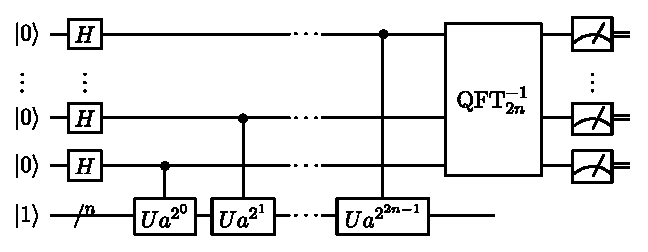
\includegraphics[width=12cm]{pic/Shor_algorithm.eps}
\caption{Circuit of Shor's algorithm}
\label{ShorAlgorithm}
\end{figure}

\subsection{Complexity}

\section{HHL algorithm}
Harrow, Hassidim, and Lloyd (HHL) algorithm approximately solves linear equation $A x = b$ where $x$ and $b$ are $n$ dimensional vectors and $A$ is a $n x n$ hermitian matrix of complex numbers. The problem would be solved if we knew the orthonormal eigen-vectors ${v_i}, i=1, 2, ...n$ and the eigen-values ${\lambda_i}$ of $A$ because the eigen-values of $A^{-1}$ are  ${1/\lambda_i}$. By writing vector $b$ in terms of the eigen-vectors $b = {\sum^n}_{i=1} \beta_i v_i$, we can achieve our goal
\begin{equation}
    x = A^{-1} b = \sum^{n}_{i=1} \frac {\beta_i} {\lambda_i} v_i .
\end{equation}

Drawing from the technique used in the Deautsch's and Shor's algorithms, we need to "kick up" the eigen-values to the phases. Let's try
\begin{equation}\label{hhl-1}
    {\sum^n}_{i=1} \beta_i e^{i t \lambda_i} \keta{v_i}
\end{equation}
where $t$ is a constant to be determined soon. With the circuit of phase estimation, we then can bring the phases down to the second set of qubits
\begin{equation}\label{hhl-2}
    {\sum^n}_{i=1} \beta_i e^{i t \lambda_i} \keta{v_i} \keta{t\lambda_i}.
\end{equation}
We then apply controlled rotation gate to kick values of the second set of qubits to the $\theta$ of the third set of qubits, which contains only one, and have
\begin{equation}\label{hhl-3}
    \sum_{i=1}^n \beta_i e^{i t \lambda_i} \keta{v_i} \keta{t\lambda_i} \keta{cos\theta_i=\frac 1 {t\lambda_i}}.
\end{equation}

\subsection{Circuit diagram}
\begin{figure}[h]\label{HHL}
\begin{quantikz}%[slice all, slice style={shorten <=8mm}, slice label style = {yshift=-38mm} ]
    \lstick{\ket{0}} & \qwbundle{1} & \qw               & \qw       & \qw       & targ{RY}  & \meter{} &\cw \rstick{} \\
    \lstick{\ket{0}} & \qwbundle{n} &\gate{H^{\otimes n}} &\ctrl{1}     & \gate{IQFT} & \ctrl{-1} & \qw &\gate{QFT} &\ctrl{1}       &\qw \rstick{Bob's 1st bit} \\
    \lstick{\ket{b}} & \qwbundle{n} & \qw               & \targ{e^{itA}} & \qw       &\qw       &\qw    &\qw       &\targ{$e^{-itA}$} & \qw \rstick{{\ket{x}}}
\end{quantikz}
\caption{HHL algorithm}
\end{figure}

\subsection{Complexity}

\section{Boson sampling algorithms}

\section{Complexity}

\section{Noise, and error correction}
\section{Channel capacity}
According to Shannon theorem, under noise, the channel capacity is $C = 2B (1+SNR)$.

\chapter*{Appendix: Quantum devices}\label{A-qubit}
\section{Types of waves}
Communication requires waves to propagate from one place to a remote place. Quantum computer qubits require stationary waves. By the propagation characteristics, we can differentiate waves into propagating waves, standing waves and trapped waves.

Radio-frequency (RF) electromagnetic waves are used for mobile communications including Wi-Fi. They can spread everywhere unless blocked or confined by reflective matters. Light waves -- electromagnetic waves with wavelength ranging from sub-micron to a few microns -- are used for optical communications. They can be channeled by optical waveguides such as optical fibers to explore different paths. They are confined in two dimensions -- the lateral dimensions -- but propagate in the dimension along the axes of the waveguides or fibers. Propagating waves are not ideal for building qubits for quantum computing. However, there have been clever designs that construct quantum computing circuits entirely using integrated optical waveguides.

Without confinement, a wave can propagate throughout space and time and does not have definite size or location. If an electromagnetic wave is confined in three dimensions, such as in a microwave oven, the wave cannot propagate anywhere other than being reflected back and forth within the confinement. And only standing waves of specific frequencies can exist. The allowed frequencies are discrete. Standing waves are good for storing information. Superconductor qubits are constructed using standing waves of electrons, as described below. Standing waves may be best visualized and understood through the vibration of a guitar string. When a string is plucked, the propagation of the vibrations is stopped and reflected by the two fixed ends. Only the waves whose phases coincide after a complete round trip of reflection survive, while the other waves cancel each other out and are suppressed.

Another type of waves, which we may call trapped waves, is not confined by anything with boundaries but is instead trapped by forces extending to infinity. Electrons in an atom are trapped waves due to the electric force of the nucleus' positive charges. The waves extend to infinity but are concentrated within a nanometer around the nucleus. Trapped waves are also good for storing information. Trapped-ion and neutral-atom qubits are built by trapped electron waves.

\section{Devices using polarization modulation}
Polarization is the vibration direction of a wave. The polarization of an electron wave is called spin and is measurable by applying a magnetic field. The polarization of an electromagnetic wave is perpendicular to its direction of propagation. The angle of polarization $\theta$ can be used to represent information in addition to the wave's phase $\phi$. Many textbooks use electron spin qubits as examples. However, such type of qubits has not been adopted by practical experiments or products until recently\cite{nanotube} because of the difficulty of building spin manipulating devices.

Physicists have studied polarization of lights for hundreds of years, and along with engineers have developed all sorts of polarization-manipulating devices. Combination of polarization and phase modulation has been widely used in communication. The dominating modulation for free-space communication and optical fiber communication in recent decades is dual polarization quadrature phase shift keying (DP-QPSK). Free space communication is mostly used for satellite-satellite communication in space. There is no substance in space to degrade the power of light waves. Free space communication can also be used for ship-ship and building-building communication on earth if the distance is not too far. Optical fiber communication is the fastest and cheapest choice for any wired communication of distance 100 meters or longer. The dominant modulation for long-distance optical fiber communication is also DP-QPSK.

Qubits for optical quantum communication naturally use the combination of polarization and phase modulation. Optical qubits have also been demonstrated in laboratories for quantum computing. Gates require manipulating wave polarization. They use optically transparent birefringent materials that have different speeds for lights of different polarization. Placing such a material in a light generator e.g. a laser, generation of light in one polarization direction is favored while the others are suppressed. A half-wave plate made from such a crystal can change the polarization angle of a light to any direction. Fig. \ref{Polarization-splitter} is a type of prism that can split the horizontal and vertical polarization components of a light that has off-angle polarization.

Fig. \ref{Demodulator-DP2} shows the functional diagram of a measurement gate. In communication term, it may be called a demodulator. The input wave from an output qubit is split into two perpendicular polarizing waves. Each wave is further split two waves of 90-degree phase difference. A single-photon dector is placed at the end of each wave. Because there is only one quantum of energy of the wave, only one electron in one of the detectors resonates with the wave and registers electric current. From this detector, we can deduce the modulation point as shown in Fig. \ref{Demodulator-DP2}.

\begin{figure}[h]
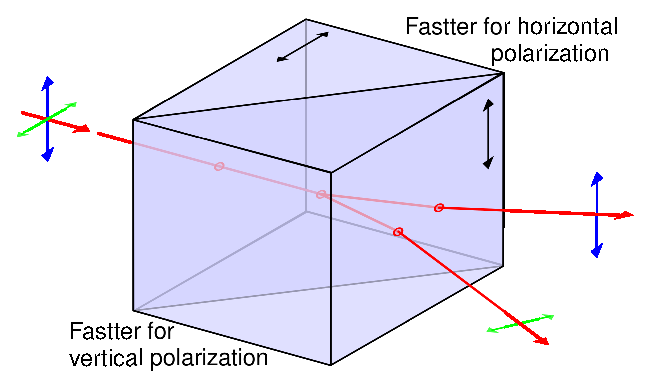
\includegraphics[width=10cm]{pic/polarization-prism.eps}
\caption{Polarization $cos{\theta} \keta{0} + e^{i \phi} sin{\theta} \keta{1}$}
\label{Polarization-splitter}
\end{figure}

\begin{figure}\label{Demodulator-DP2}
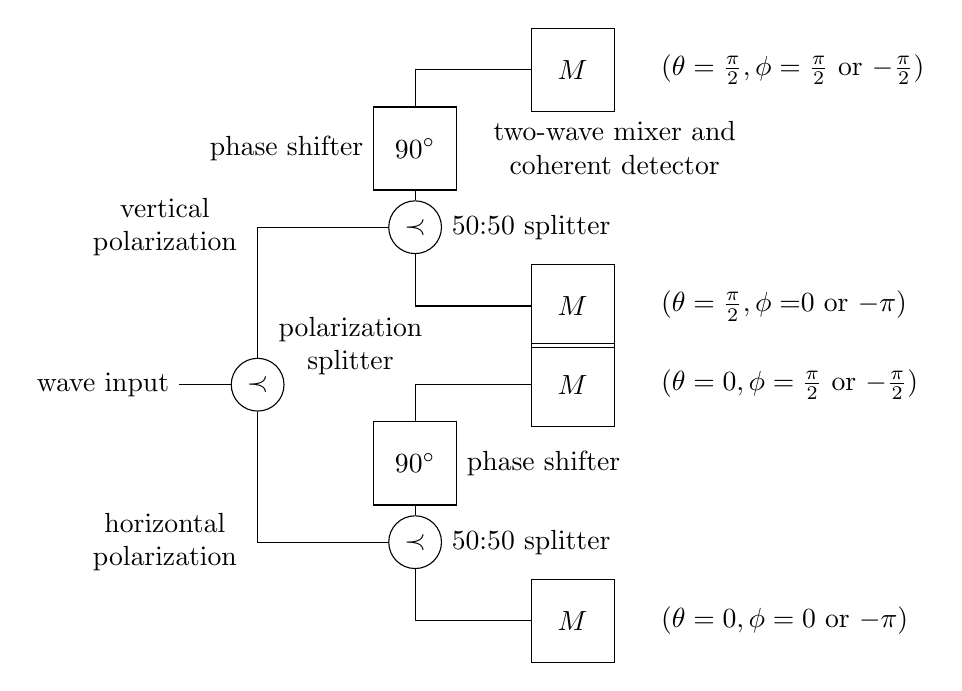
\begin{tikzpicture}[scale=1]
    \path
    (-3,0) node[anchor=east] (input) {wave input}
    (-2,0) node[circle, draw=black] (split) {$\prec$}
%    (-2,1) node[Gate] (theta90) {$90^\circ$}
    (0,2) node[circle, draw=black] (tsp) {$\prec$}
    (0,-2) node[circle, draw=black] (bsp) {$\prec$}
    (0,3) node[Gate] (tphi90) {$90^\circ$}
    (0,-1) node[Gate] (bphi90) {$90^\circ$}
    (2,4) node[Gate] (td1) {$M$}
    (2,1) node[Gate] (td2) {$M$}
    (2,0) node[Gate] (bd1) {$M$}
    (2,-3) node[Gate] (bd2) {$M$};
     
    \path (3,4) node[anchor=west] (bit11) {$(\theta=\frac \pi 2, \phi=\frac \pi 2$ or $-\frac \pi 2)$}
    (3,1) node [anchor=west] (bit10) {$(\theta=\frac \pi 2, \phi=$0 or $-\pi)$}
    (3,0) node [anchor=west] (bit01) {$(\theta=0, \phi=\frac \pi 2$ or $-\frac \pi 2)$}
    (3,-3) node [anchor=west] (bit00) {$(\theta=0, \phi=0$ or $-\pi)$}
    (-2,2) node [text width=60, align=center, anchor=east] (V) {vertical polarization}
    (-2,-2) node [text width=60, align=center, anchor=east] (H) {horizontal polarization};

    \draw (input) -- (split) |- (tsp) -- (tphi90) |- (td1);
    \draw (split) |- (bsp) -- (bphi90) |- (bd1);
    \draw (tsp) |- (td2);
    \draw (bsp) |- (bd2);
    \draw (split) node[text width=60, align=center, anchor=south west] {polarization splitter};
    \draw (tsp.east) node[anchor=west] {50:50 splitter};
    \draw (bsp.east) node[anchor=west] {50:50 splitter};
    \draw (tphi90.west) node[anchor=east] {phase shifter};
    \draw (bphi90.east) node[anchor=west] {phase shifter};
    \draw (td1.south east) node[text width=90, align=center, anchor=north] {two-wave mixer and coherent detector};
\end{tikzpicture}

    \caption{Polarization qubit demodulator}
\end{figure}

\section{Devices using optical waveguides}
Waveguides confine waves in two dimensions and allowing them to propagate in once dimension. Optical fibers are the mostly deployed. A couple of decades ago, radio-frequency cables for broadcasting TV signals were mostly deployed.
Another type of qubits uses lights confined in optical waveguides. Optical fiber is a type of waveguide. We use the optical wave in the waveguide on the left in Fig. \ref{Fiber} to encode the binary number 0 and label it $\keta{0}$. We use the one in waveguide on the right to encode 1 and label it $\keta{1}$. The two waves have the same frequency and amplitude. They don't overlap and are of course orthogonal to each other. If we bring the two waveguides together to overlap (using an optical coupler), we get a superposition wave that is a sum of both waves. If the sum has $cos\theta$ amount in amplitude from $\keta{0}$ wave contributes and $sin\theta_p$ amount in amplitude from the $\keta{1}$ wave, we can use the value $\theta_p$ to characterize the superposition wave.

\begin{figure}[h]\label{Fiber}
%\includegraphics[width=6cm]{pic/wguideQubit.png}
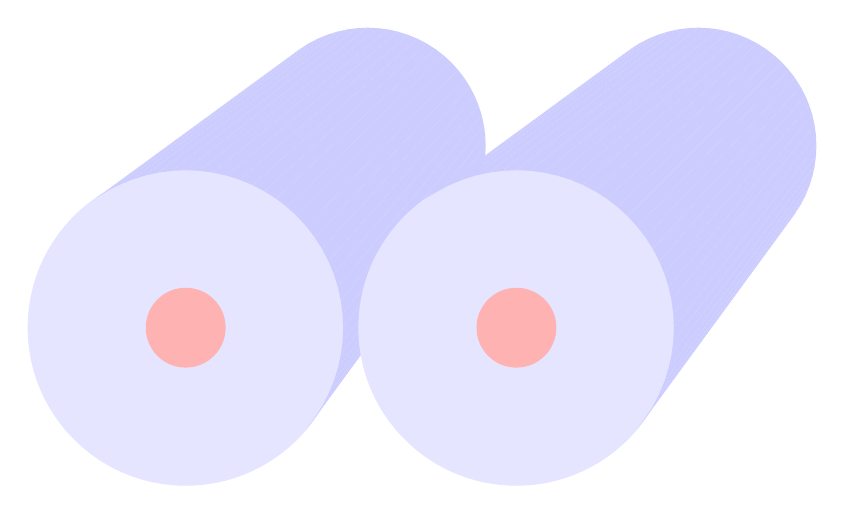
\begin{tikzpicture}[scale=0.5]
    \def\R{4} % Outer radius
    \def\Rb{3} % Outer radius
    \def\r{1} % Inner radius
    \def\L{6} % Half Length of the tube
    \def\S{4.2} % half Shift distance between tubes/fibers
    \def\I{5} % increment

    % Left tube
    \draw[blue!10,fill] (-\S,0,\L) circle (\R);   
    \draw[red!30,fill] (-\S,0,\L) circle (\r);    
    %\draw[decorate,decoration=zigzag] (-\S,0,-\L) circle (\Rb);
    \foreach \t in {-40,-35,...,123} {
        \fill[blue!20] ({\R*cos(\t+\I)-\S}, {\R*sin(\t+\I)}, \L) -- ({\R*cos(\t)-\S}, {\R*sin(\t)}, \L) 
        -- ({\Rb*cos(\t)-\S}, {\Rb*sin(\t)}, -\L) -- ({\Rb*cos(\t+\I)-\S}, {\Rb*sin(\t+\I)}, -\L) -- cycle;
    }

    % Right tube    
    \draw[blue!10,fill] (\S,0,\L) circle (\R);   
    \draw[red!30,fill] (\S,0,\L) circle (\r);    
    %\draw[black!10] (\S,0,-\L) circle (\Rb);
    \foreach \t in {-40,-35,...,123} {
        \fill[blue!20] ({\R*cos(\t+\I)+\S}, {\R*sin(\t+\I)}, \L) -- ({\R*cos(\t)+\S}, {\R*sin(\t)}, \L) 
        -- ({\Rb*cos(\t)+\S}, {\Rb*sin(\t)}, -\L) -- ({\Rb*cos(\t+\I)+\S}, {\Rb*sin(\t+\I)}, -\L) -- cycle;
    }
\end{tikzpicture}
\caption{A waveguide qubit comprised by two single-mode optical fibers $cos{\theta} \keta{0} + e^{i \phi} sin{\theta} \keta{1}$}
\end{figure}

The Xanadu.ai M-8 quantum computing chip assembles waveguide qubits and processing gates in an integrated waveguide circuit. We see it very much resembles a maze. The optical waveguides are the paths that light waves traverse. Its couplers and splitters resemble the junctions of maze. A coupler merge two light paths into one, and a splitter split one into two. The chip has 8 entrances and 8 exits and can build $8^8$ possible paths.

\section{Superconductor qubits}
A superconductor transmon qubit is similar to the string of a guitar and uses the first two standing waves, which resonate at the first and second harmonic frequencies respectively, to represent the integers of "0" and "1". Such a qubit is constructed by two superconductors separated by a layer of insulator. The insulator is thin enough for electrons to move ("tunnel") back and forth from one superconductor to another without loss of energy. But traveling through the insulator leads to delays (phase delays) of the electrons. The back-and-forth movement (vibration) of the electrons between the two superconductors resonate as standing waves at periods fractions of the delay. typically, the first fundamental frequency and the first harmonic are used to represent "0" and "1".
\begin{figure}[h]
\includegraphics[width=12cm]{pic/supercQubit.jpg}
\caption{Josephson junction}
\label{Superconductor}
\end{figure}

\begin{figure}[h]
\includegraphics[width=12cm]{pic/superGates.jpg}
\caption{Superconductor gates.}
\label{superGates}
\end{figure}

\section{Trapped atoms and ions}

\begin{figure}[h]
\includegraphics[width=12cm]{pic/h-atom.png}
\caption{Atom}
\label{Atom}
\end{figure}

%\backmatter

\addcontentsline{toc}{chapter}{Bibliography}
\chapter*{Bibliography}
\bibliographystyle{unsrt}
   \bibliography{qcc}

\addcontentsline{toc}{chapter}{Index}
\printindex
\end{document}